% Topic #2 - Science

%------------------------------------
% Main Settings
%------------------------------------
\documentclass[10pt]{beamer}

%--------------------------------------%
% Set font, and frame title info    %
%--------------------------------------%
\usefonttheme{serif}
\setbeamerfont{frametitle}{series=\bfseries}
\setbeamerfont{framesubtitle}{series=\bfseries}

%--------------------------------------
% "Sub-settings"
%--------------------------------------
\setbeamertemplate{navigation symbols}{}		% Get rid of navigation symbols
\setbeamertemplate{items}[default]				% Uses triangles and numbers instead of 3D balls (which I don't like)
\setbeamertemplate{itemize items}[circle]		% Use circles instead of triangles for itemized lists

%-------------------------------------
% Custom Commands
%-------------------------------------
\newtheorem{hypothesis}{Hypothesis}

%---For Footnotes---%
\usepackage{tikz}
\usepackage[absolute,overlay]{textpos}
\usetikzlibrary{calc,shapes.callouts,shapes.arrows,shapes,positioning}
\newenvironment{reference}[2]{%
	\begin{textblock*}{\textwidth}(#1,#2)
		\tiny\bgroup\color{gray}}{\egroup\end{textblock*}}
%------%		

%----------------------------------------%
% For making definitions in boxes        %
%----------------------------------------%
\usepackage{tcolorbox}

%--- For links ---%
\usepackage{hyperref}

%-- Packages for making nice tables --%
\usepackage{booktabs}
\usepackage{makecell}  % Required for specifying multiple rows within a table cell

%--------------------------------%
%     Custom Colours             %
%--------------------------------%
\usepackage{xcolor}
\definecolor{myblue}{rgb}{0,0.3,0.6}
\definecolor{myblue2}{rgb}{0,0.4,0.8}
\setbeamercolor{frametitle}{fg=myblue}
\setbeamercolor{framesubtitle}{fg=myblue2}
\setbeamercolor{itemize item}{fg=myblue}
\setbeamercolor{itemize subitem}{fg=myblue2}
\setbeamercolor{enumerate item}{fg=myblue}
\setbeamercolor{enumerate subitem}{fg=myblue2}


%----------------------------------%
% Creating nice blocks             %
%----------------------------------%
\setbeamercolor{block title}{bg=myblue, fg=white} %bg=background, fg=foreground
\setbeamercolor{block body}{bg=myblue!20, fg=black} %bg=background, fg=foreground
\setbeamerfont*{block title}{family=\sffamily, series=\bfseries, size=\large}
\setbeamertemplate{blocks}[rounded][shadow=true]


%------------------------%
% For making callouts    %
%------------------------%
\tikzset{
  notice/.style  = { draw, rectangle callout, callout relative pointer={#1} },
}

%------------------------------------------
%  Begin Presentations
%------------------------------------------
\begin{document}


%-----------------------%
%  Title Slide          %
%-----------------------%
\begin{frame}
	\begin{tikzpicture}[remember picture,overlay]
		\fill[color=myblue, draw=none] (current page.west) rectangle(current page.north east);
		\node at (4.5, 0.2) {\color{white}\LARGE{\textbf{Science \& the Scientific Method}}};
	\end{tikzpicture}
\end{frame}


%-----------------------%
% Scientific Literacy I %
%-----------------------%
\begin{frame}[t]
\frametitle{Scientific Literacy is in Trouble}
\vspace{0.5cm}

	\begin{reference}{4mm}{92mm}
		\rule{1.5cm}{0.25pt}\\
		1. Miller (1998) \emph{Public Understanding Sci}. \textbf{7}: 203--223.
	\end{reference}
	
	Only 20--25\% of North Americans are scientifically literate!$^{1}$
	
	\vspace{0.5cm}
	
		\begin{columns}
			\begin{column}{0.6\textwidth}
				\begin{itemize}
					\item 1 in 5 think the Sun revolves around the Earth
					\medskip
					\item $<$ 1/3 know DNA is the hereditary material
					\medskip
					\item $\sim$10\% know what radiation is
					\medskip
					\item \ldots
				\end{itemize}
			\end{column}
			
			\begin{column}{0.4\textwidth}
				\begin{center}
					
\includegraphics[width=0.8\textwidth]{figures/mooney.jpg}
				\end{center}
			\end{column}
		\end{columns}
\end{frame}


%------------------------%
% Scientific Literacy II %
%------------------------%
\begin{frame}
\frametitle{Scientific Literacy is in Trouble}

	\begin{columns}
		\begin{column}{0.7\textwidth}
			\begin{center}
				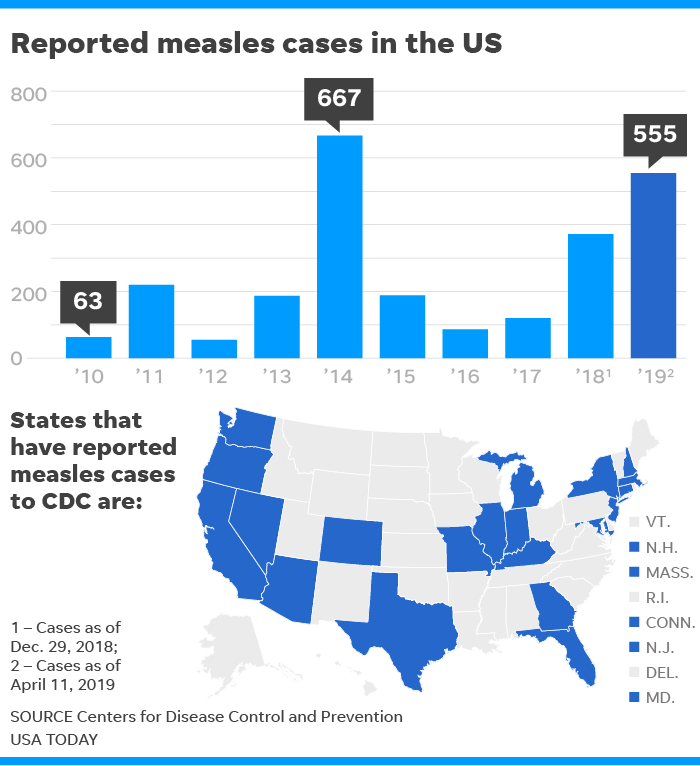
\includegraphics[width=0.8\textwidth]{figures/measles.png}
			\end{center}
		\end{column}
		
		\begin{column}{0.3\textwidth}
			\begin{center}
				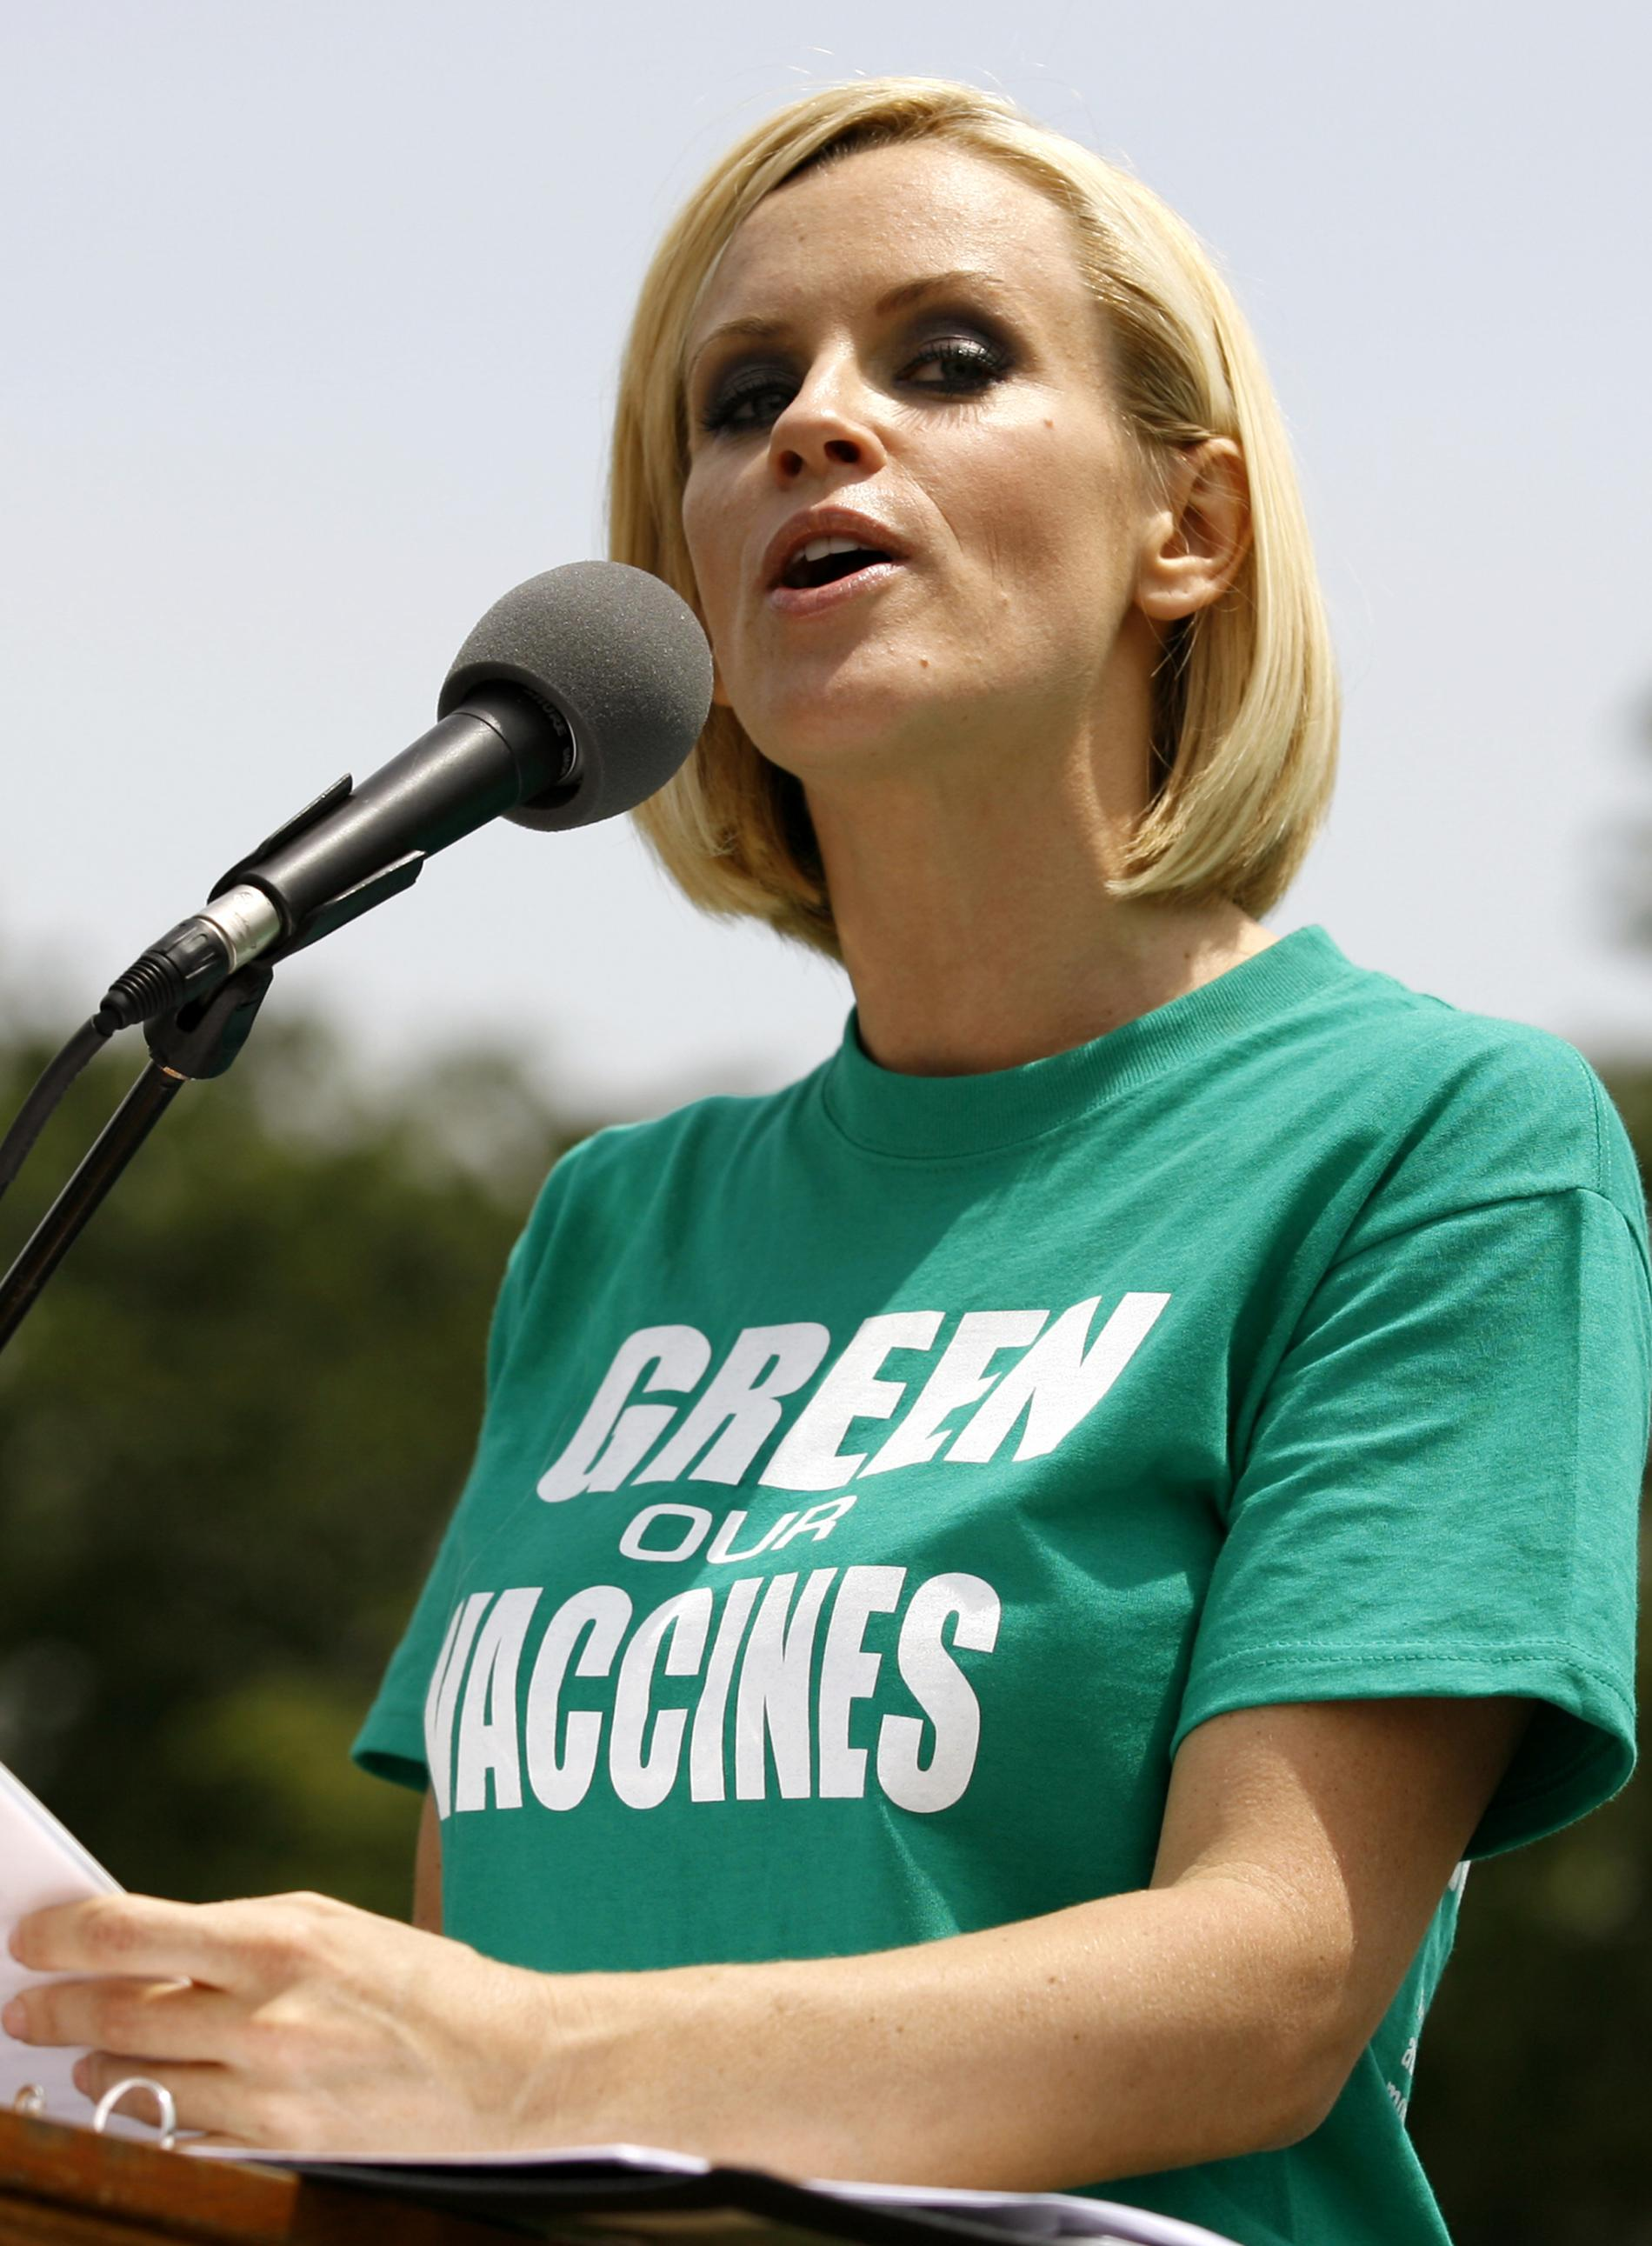
\includegraphics[width=0.8\textwidth]{figures/jenny.jpg}
			\end{center}
		\end{column}
	\end{columns}
\end{frame}


%-------------------------%
% Scientific Literacy III %
%-------------------------%
\begin{frame}[t]
\frametitle{Why Is Scientific Literacy Important?}
\vspace{0.5cm}

	Science is playing an increasing role in our day-to-day lives\\
		\begin{itemize}
			\item Climate change
			\medskip
			\item Alternative energy sources
			\medskip
			\item Health care
			\medskip
			\item Impact of development
			\medskip
			\item Disease spread (vaccines, HIV, resistant bacteria)
			\medskip
			\item Stem cell research
			\medskip
			\item Forensics
			\medskip
			\item \ldots
		\end{itemize}
\end{frame}


%----------------------------%
% The Scientific Method I    %
%----------------------------%
\begin{frame}[t]
\frametitle{The Scientific Method}
	
	\begin{tikzpicture}[overlay]
		\node[draw=myblue2, fill=myblue2!30, rounded corners, minimum width=2.5cm, minimum height = 0.75cm] at (7, -0.5) (node1) {Observations};
		\node[draw=myblue2, fill=myblue2!30, rounded corners, minimum width=2.5cm, minimum height = 0.75cm] at (7, -2.5) (node2) {Hypotheses};
		\node[draw=myblue2, fill=myblue2!30, rounded corners, minimum width=2.5cm, minimum height = 0.75cm] at (7, -4.5) (node3) {Predictions};
		\node[draw=myblue2, fill=myblue2!30, rounded corners, text width = 2.5cm, align = center, minimum width=2.5cm, minimum height = 0.75cm] at (7, -6.5) (node4) {\footnotesize{Experiments or New Observations}};
		\node[draw=gray, fill=gray!30, rounded corners, text width = 3.5cm, align = center, minimum width=2.5cm, minimum height = 0.75cm] at (3.0, -4.5) (node5) {\scriptsize{If results are not consistent, reject or revise the hypothesis}};
		\node[draw=red, fill=red!30, rounded corners, text width = 6.5cm, align = center, minimum width=2.5cm, minimum height = 0.75cm, rotate = 270] at (9, -3.5) (node6) {Critical Thinking};
		
		
		\draw[->, >=latex, thick, color=myblue2] (node1)--(node2);
		\draw[->, >=latex, thick, color=myblue2] (node2)--(node3);
		\draw[->, >=latex, thick, color=myblue2] (node3)--(node4);
		\draw[->, >=latex, dashed, thick, color=gray] (node4)-|(node5);
		\draw[->, >=latex, dashed, thick, color=gray] (node5)|-(node2);
	\end{tikzpicture}
\end{frame}


%----------------------------%
% The Scientific Method II   %
%----------------------------%
\begin{frame}
\frametitle{The Scientific Method}
	
	\begin{center}
		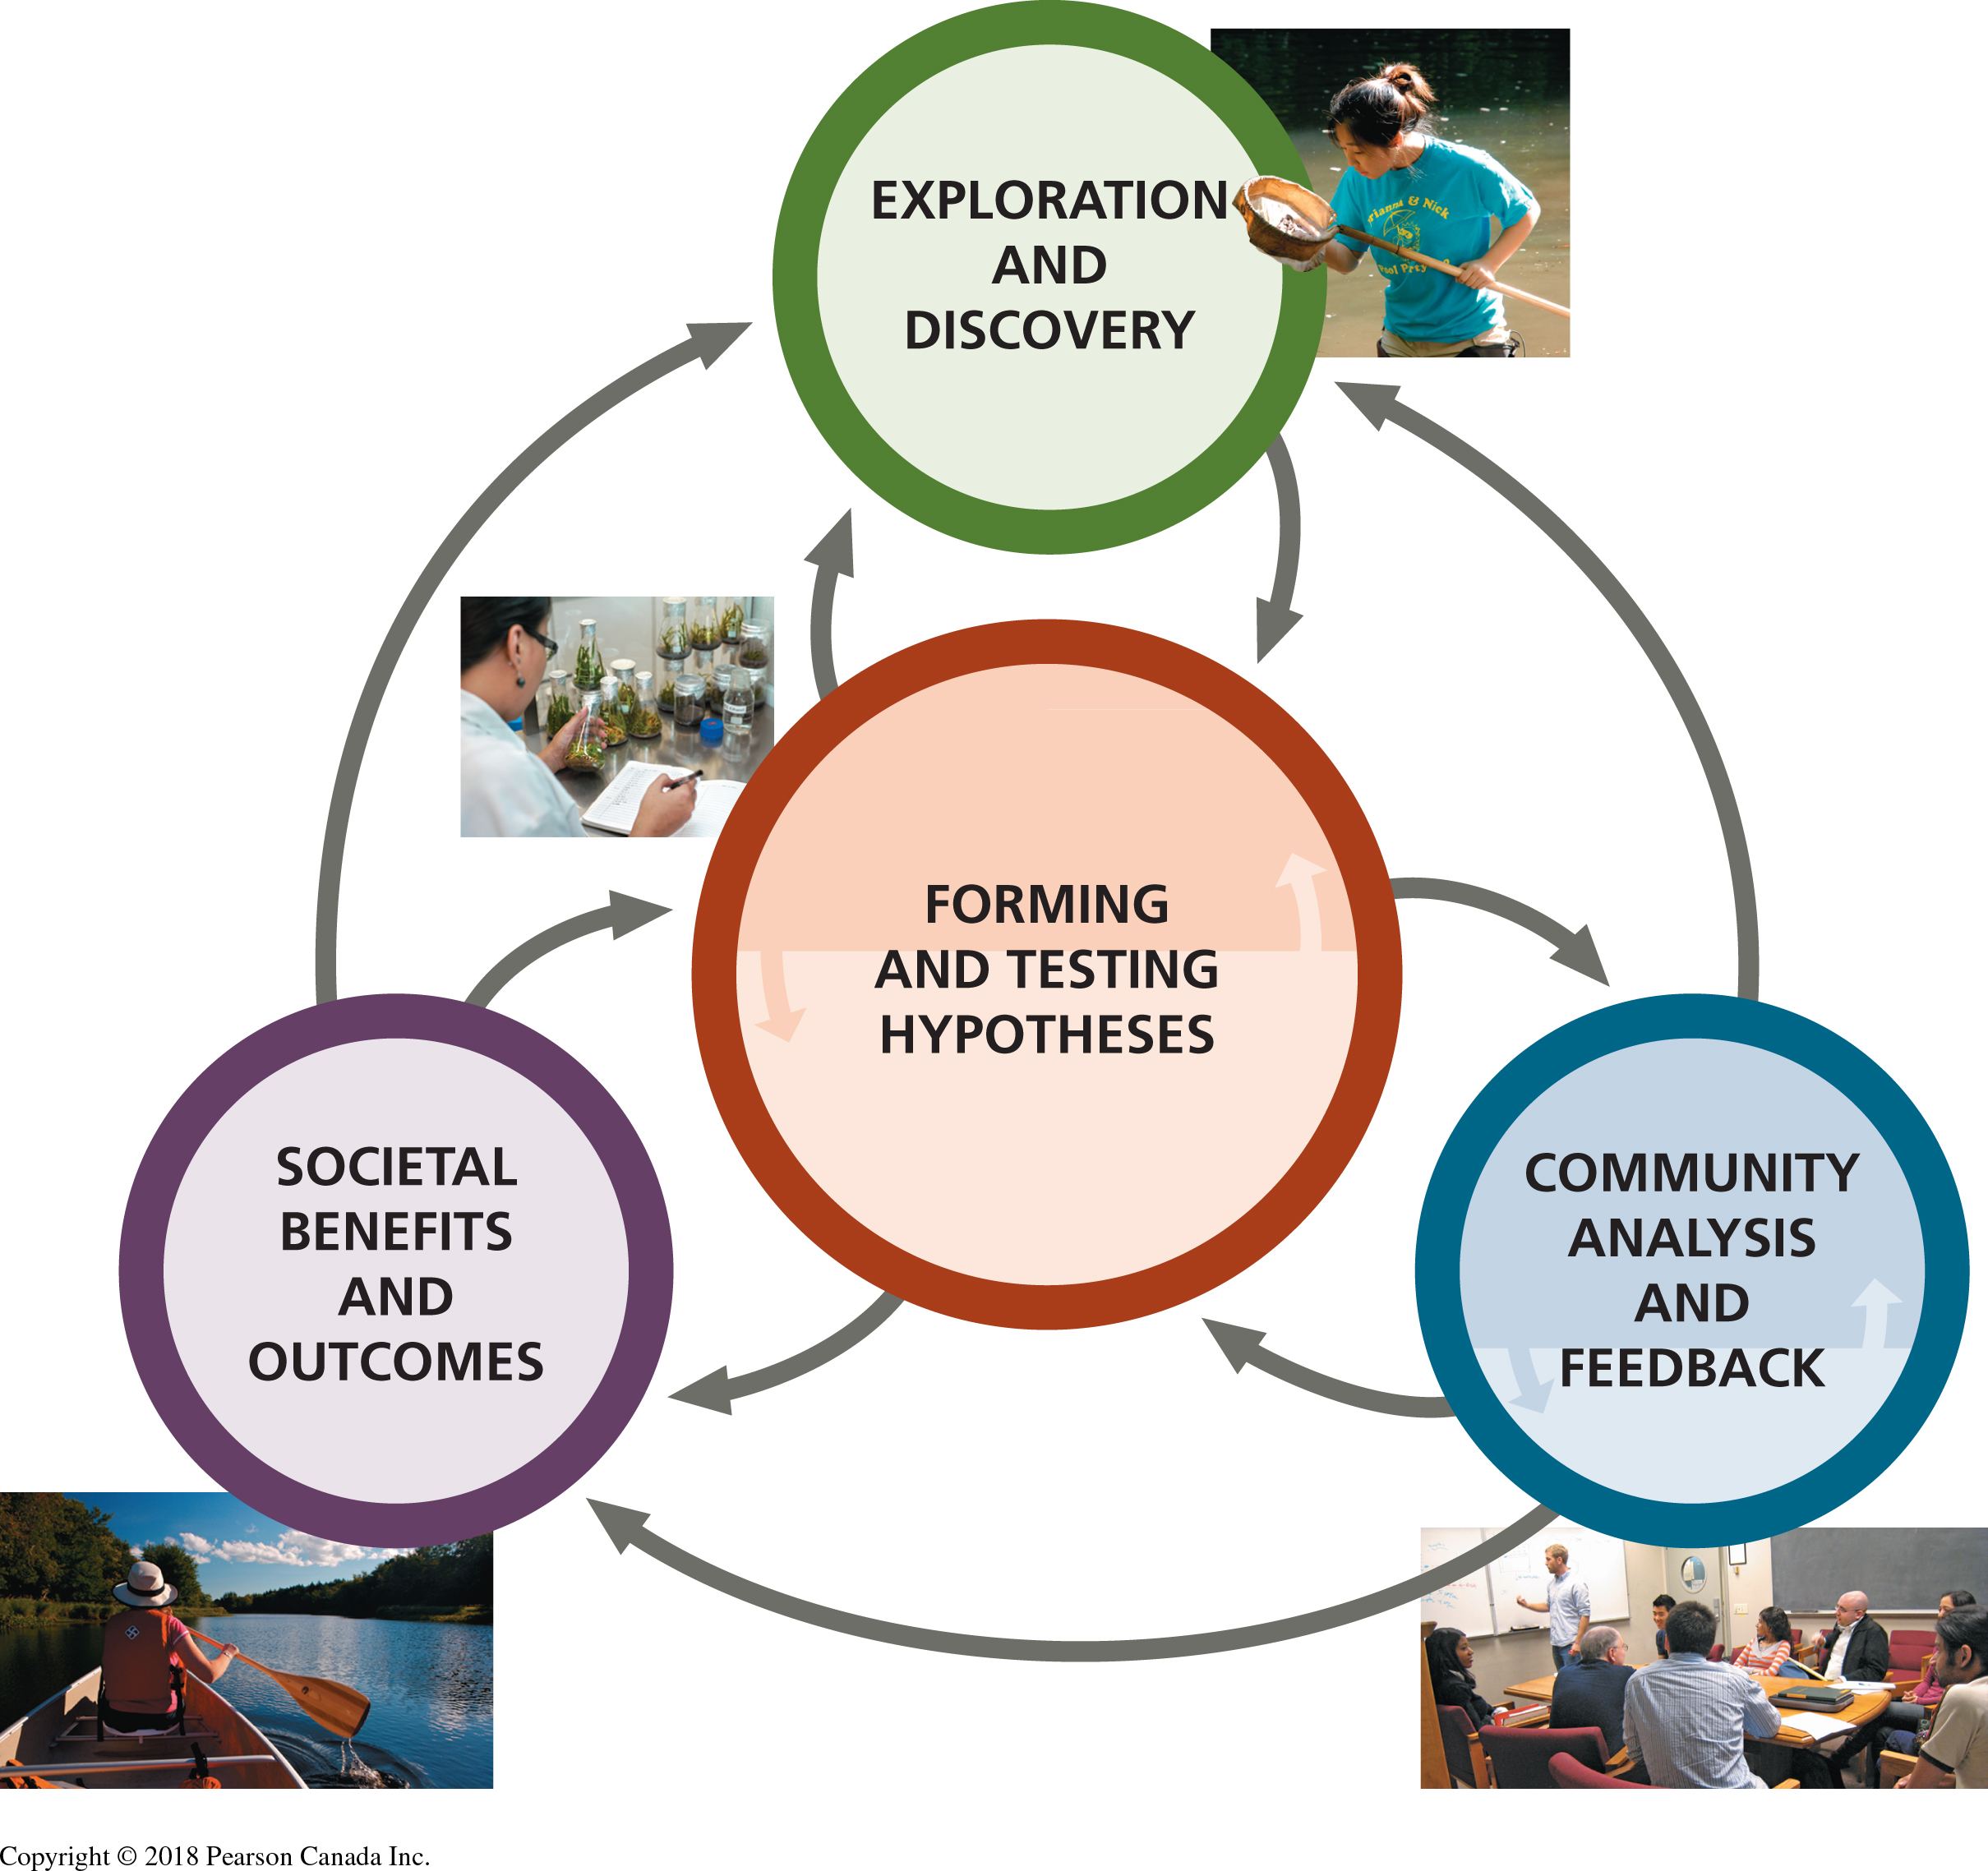
\includegraphics[width=0.6\textwidth]{figures/science.jpg}
	\end{center}	
\end{frame}


%-------------------------%
% Critical Thinking I     %
%-------------------------%
\begin{frame}[t]
\frametitle{Critical Thinking}
\vspace{0.5cm}

	In science, critical thinking often means: being able to separate \textcolor{red}{\textbf{data}} from \textcolor{red}{\textbf{interpretation of data}}
	
		\medskip
		\begin{itemize}
			\item Don't rely on other people's word or interpretation, no matter who they are
			\medskip
			\item Only trust data (and only do this if you are convinced methods were appropriate)
		\end{itemize} 

	\vspace{0.5cm}
	
	\begin{center}
		\textcolor{myblue}{Should do nothing short of changing\\ the way you interact with the world}
	\end{center}
\end{frame}


%-------------------------%
% Critical Thinking II    %
%-------------------------%
\begin{frame}[t]

	\begin{columns}[t]
		\begin{column}{0.33\textwidth}
			\begin{center}
				
\includegraphics[width=0.7\textwidth]{figures/cbc.png}\\
				\vspace{1.5cm}
				
\includegraphics[width=0.7\textwidth]{figures/60.jpg}
			\end{center}
		\end{column}
		
		\begin{column}{0.33\textwidth}
			\begin{center}
				\vspace{0.5cm}
				
\includegraphics[width=1.3\textwidth]{figures/wikipedia.png}
			\end{center}
		\end{column}
		
		\begin{column}{0.33\textwidth}
			\begin{center}
				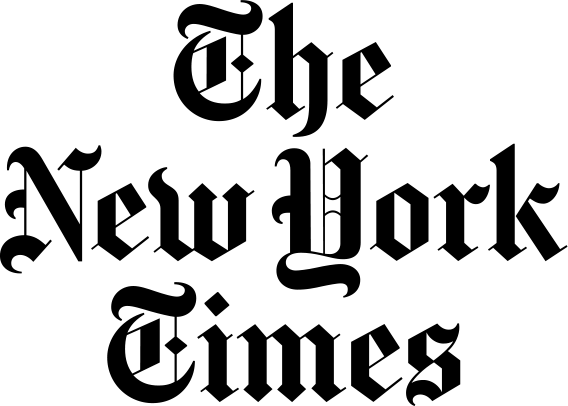
\includegraphics[width=0.7\textwidth]{figures/nyt.png}\\
				\vspace{3.5cm}
				
\includegraphics[width=0.7\textwidth]{figures/daily.png}
			\end{center}
		\end{column}
	\end{columns}
\end{frame}


%----------------------------%
%  Critical Thinking III     %
%----------------------------%
\begin{frame}
	\begin{columns}
		\begin{column}{0.5\textwidth}
			\begin{center}
				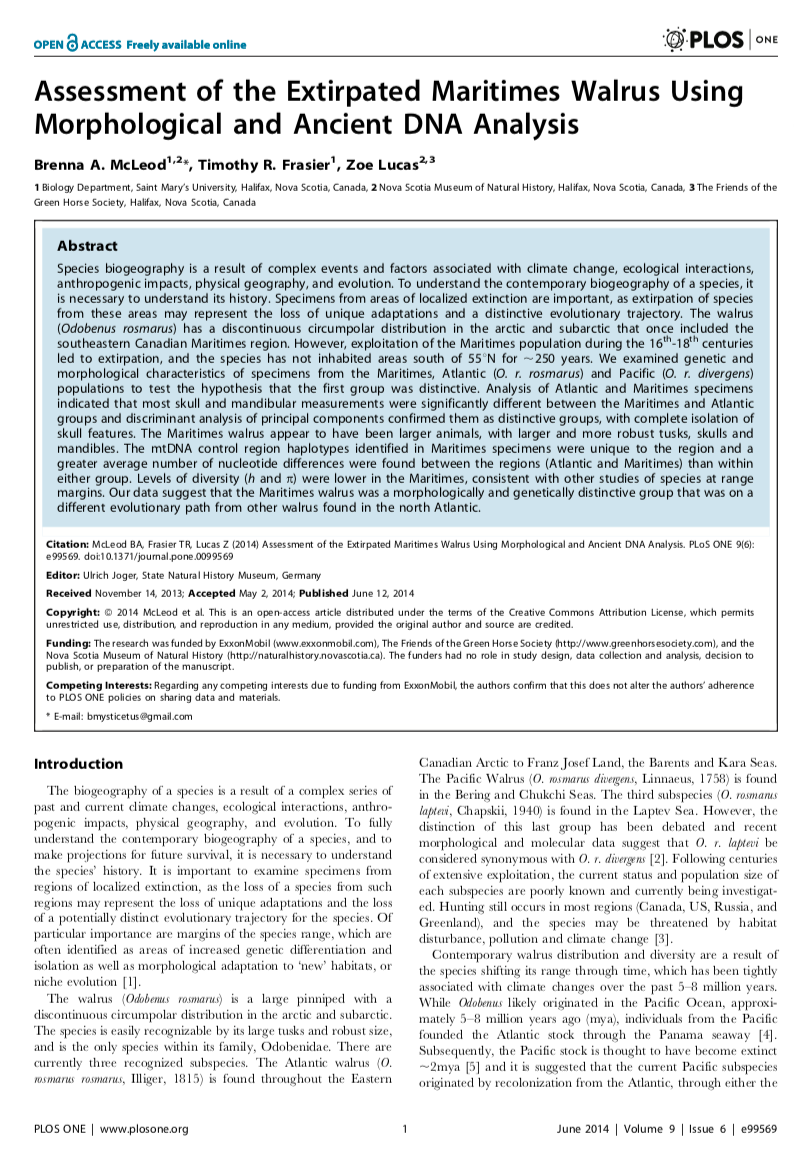
\includegraphics[width=1.0\textwidth]{figures/paper1.png}
			\end{center}
		\end{column}
		
		\begin{column}{0.5\textwidth}
			\begin{center}
				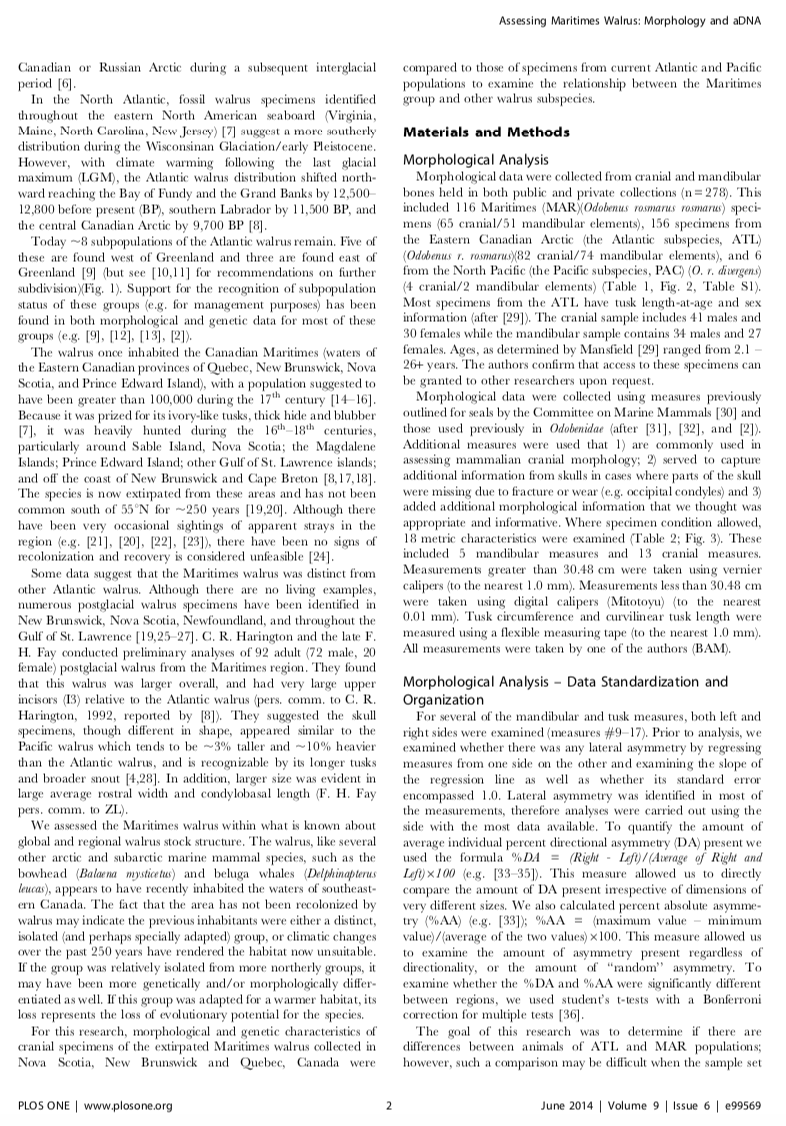
\includegraphics[width=1.0\textwidth]{figures/paper2.png}
			\end{center}
		\end{column}
	\end{columns}
\end{frame}


%----------------------------%
%  Critical Thinking IV      %
%----------------------------%
\begin{frame}
	\begin{columns}
		\begin{column}{0.5\textwidth}
			\begin{center}
				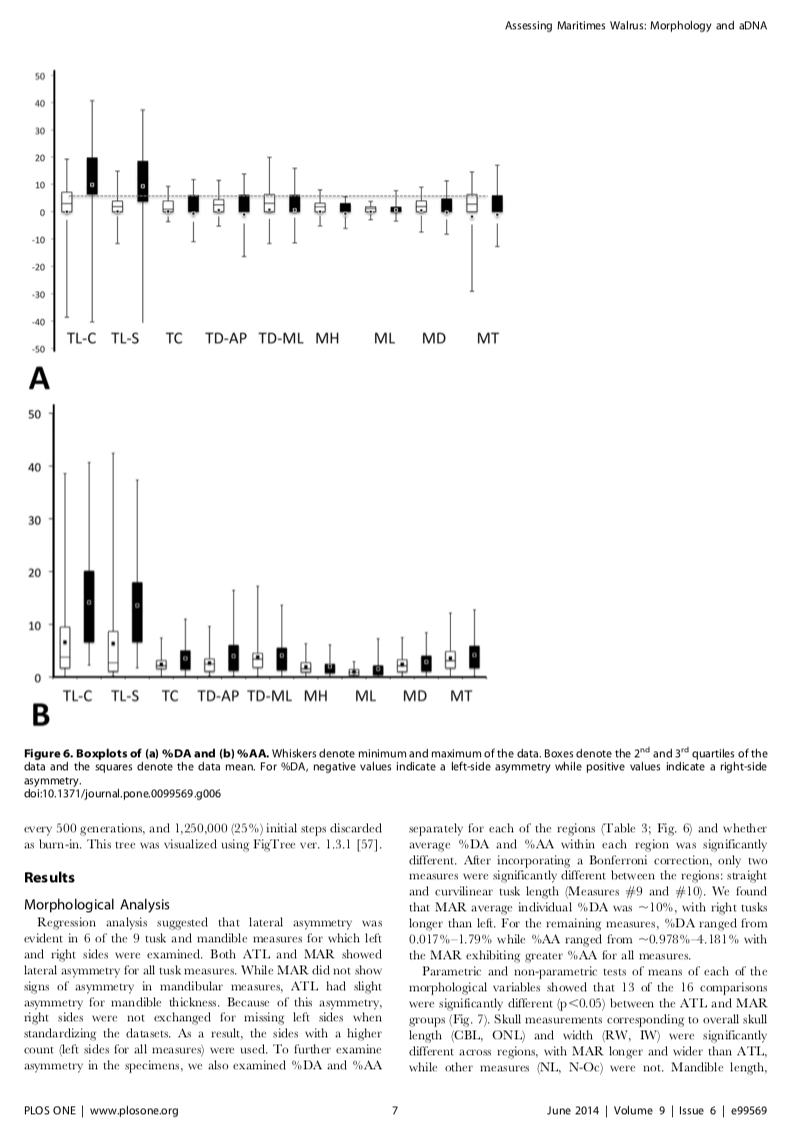
\includegraphics[width=1.0\textwidth]{figures/paper3.png}
			\end{center}
		\end{column}
		
		\begin{column}{0.5\textwidth}
			\begin{center}
				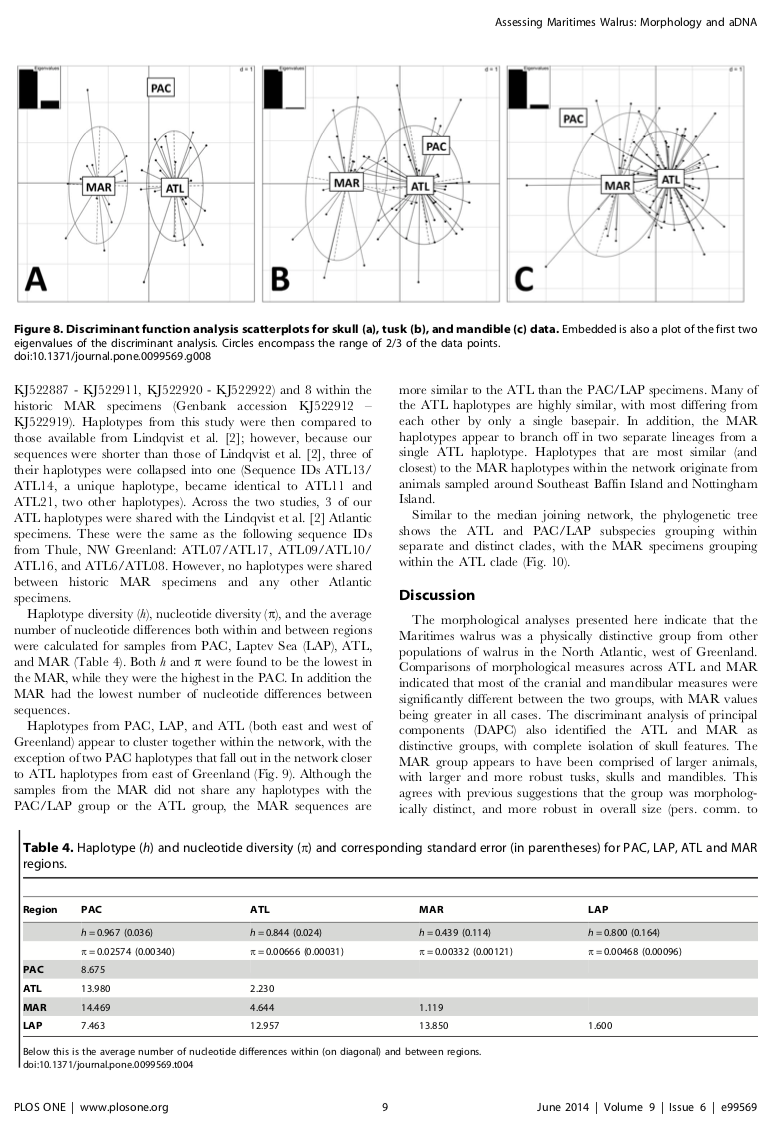
\includegraphics[width=1.0\textwidth]{figures/paper4.png}
			\end{center}
		\end{column}
	\end{columns}
\end{frame}


%--------------------------%
% How Science Works I      %
%--------------------------%
\begin{frame}[t]
\frametitle{How Science Works}
\vspace{0.5cm}

	\begin{center}
		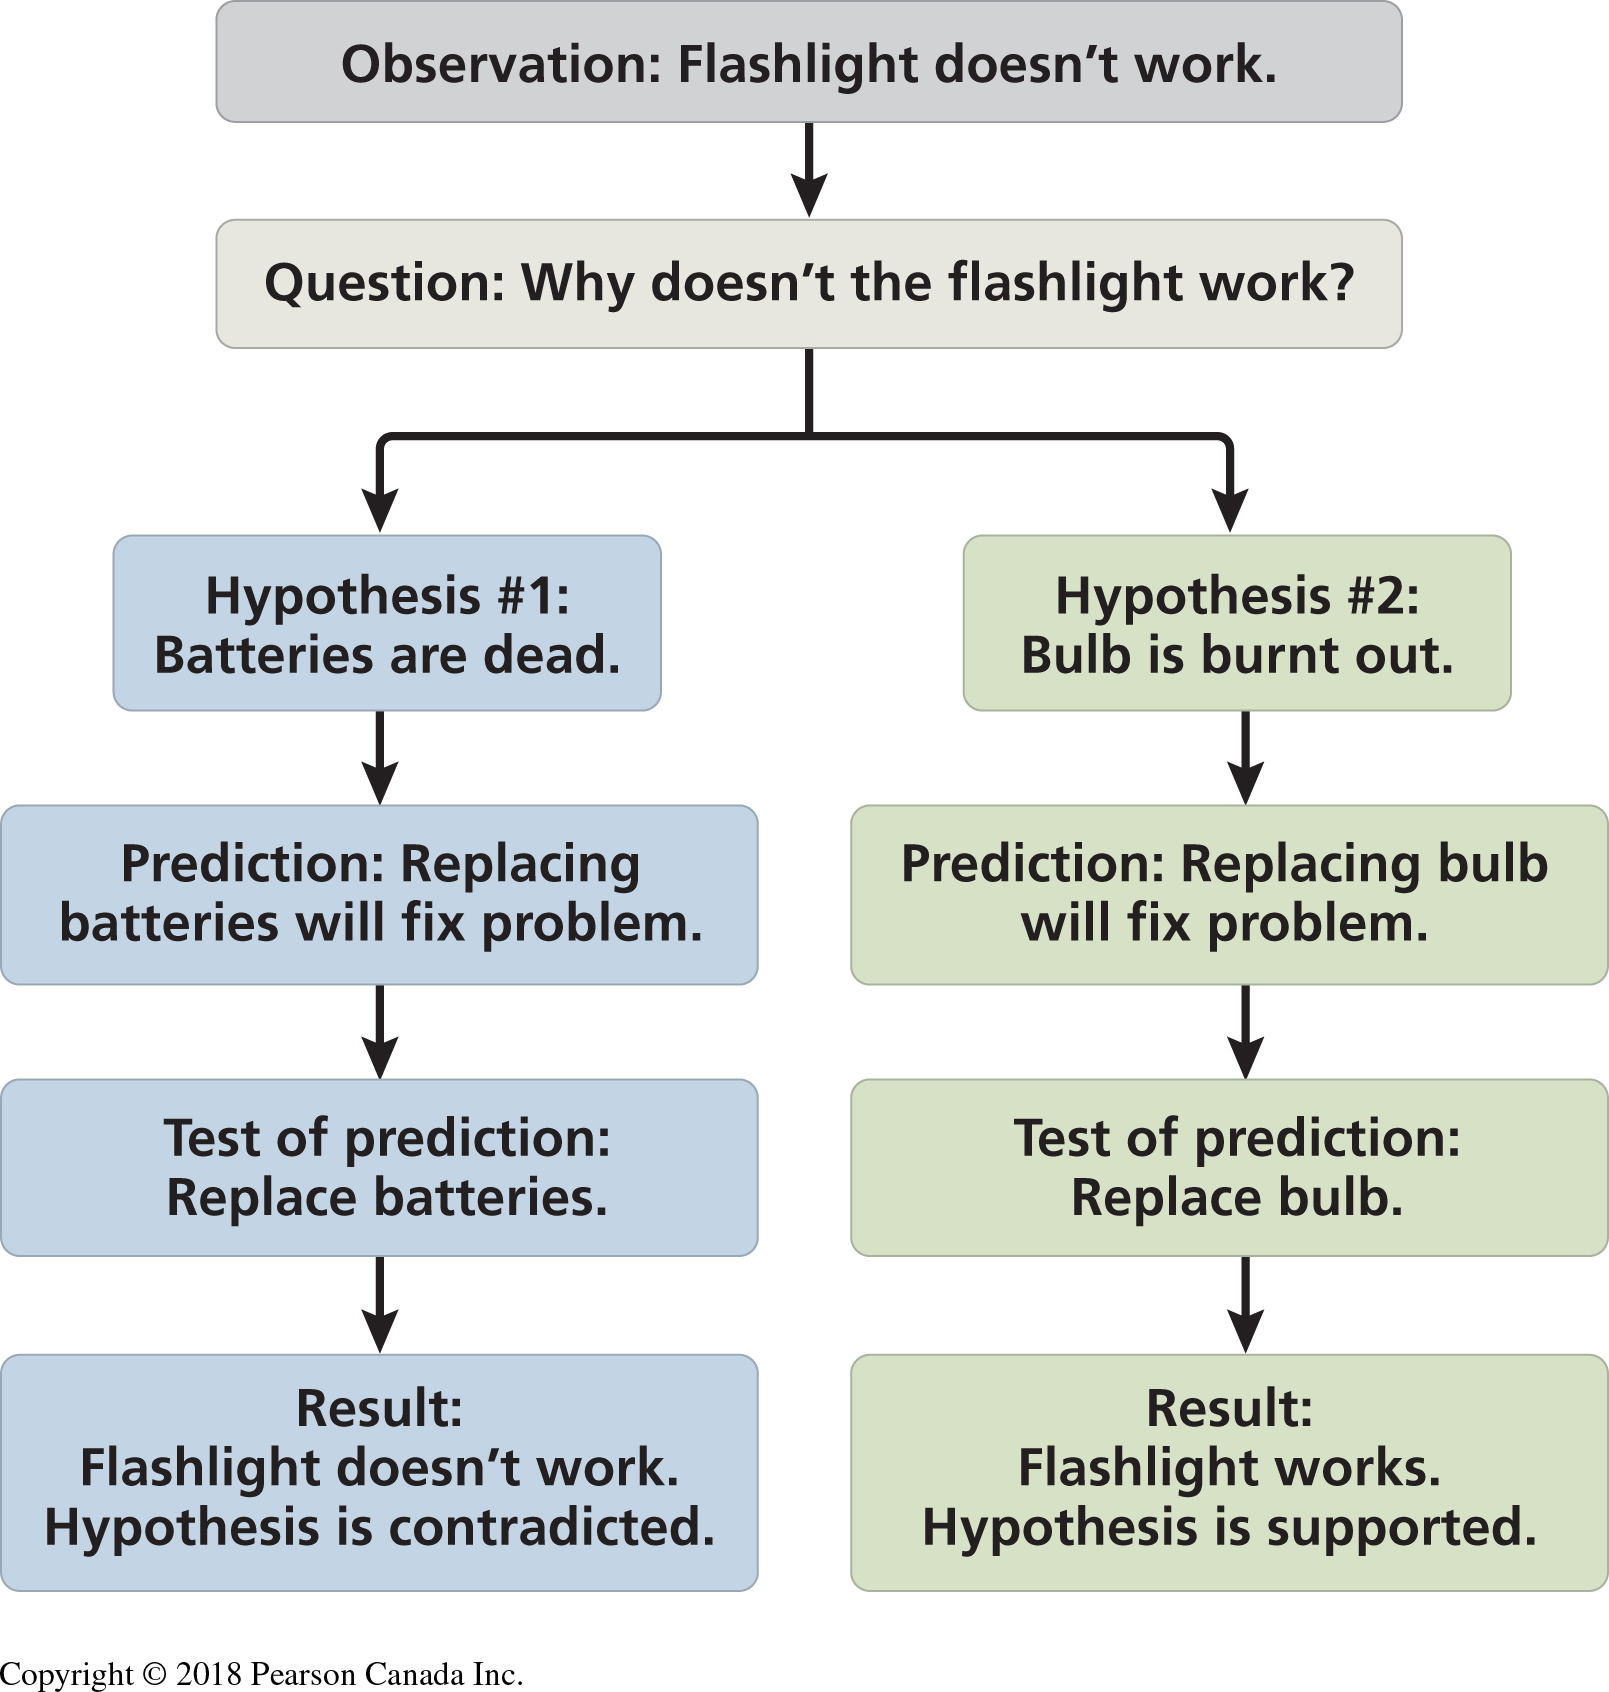
\includegraphics[width=0.6\textwidth]{figures/science2.jpg}
	\end{center}
\end{frame}


%--------------------------%
% How Science Works II     %
%--------------------------%
\begin{frame}[t]
\frametitle{How Science Works}

	\begin{tikzpicture}[overlay]
		\node[draw=myblue2, fill=myblue2!30, ellipse, text width = 2cm, align = center] at (2, -5.5) (node1) {Observations/ facts};
		
		\node[draw=myblue2, fill=myblue2!30, ellipse, minimum width=2.0cm, minimum height = 1.0cm, align = center] at (9, -5.5) (node2) {
\includegraphics[width=0.15\textwidth]{figures/nest.png}};
		
		\node at (7.0, -5.5) (node3) {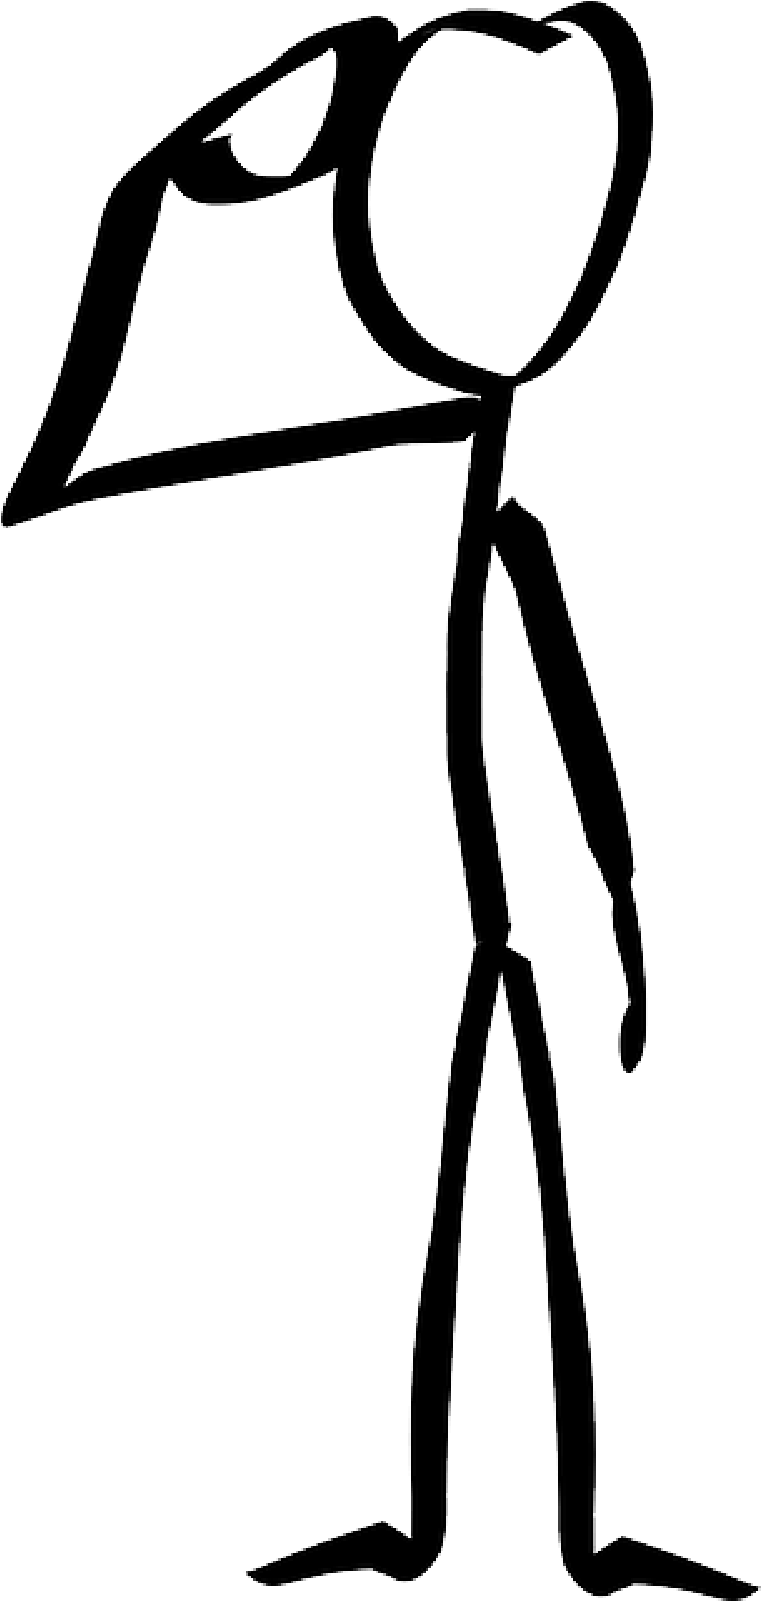
\includegraphics[width=0.10\textwidth]{figures/stick.png}};
		
		\node[notice={(-0.5, -0.3)}, overlay, ellipse callout, text width=2.5cm, align = center] at (9.3, -3.2) (node4) {\scriptsize{The average eggs/nest for species X is 3. \textcolor{red}{I wonder why}}};
	\end{tikzpicture}
\end{frame}


%--------------------------%
% How Science Works III    %
%--------------------------%
\begin{frame}
\frametitle{How Science Works}
	
	\begin{tikzpicture}[overlay]
		\node at (2, -0.3) (node1) {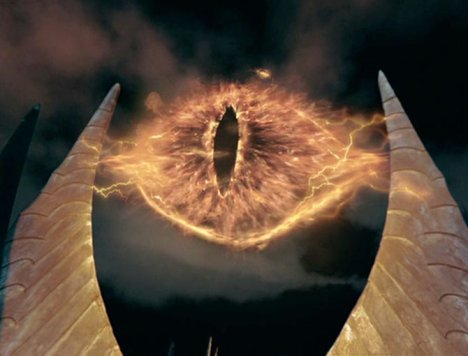
\includegraphics[width=0.35\textwidth]{figures/eye.jpg}};
		\node at (9, -0.3) (node2) {
\includegraphics[width=0.35\textwidth]{figures/teacher.png}};
		
		\node[notice={(-0.5, -0.3)}, overlay, ellipse callout, text width=2.0cm, align = center] at (4, 2) (node4) {\scriptsize{That's the way I wanted it}};
		\node[notice={(0.4, -0.3)}, overlay, ellipse callout, text width=2.0cm, align = center] at (7, 3) (node4) {\scriptsize{3 is the optimal number of population growth}};
	\end{tikzpicture}
\end{frame}


%--------------------------%
% How Science Works IV     %
%--------------------------%
\begin{frame}
\frametitle{How Science Works}
	
	\begin{tikzpicture}[overlay]
		\node at (2, -0.3) (node1) {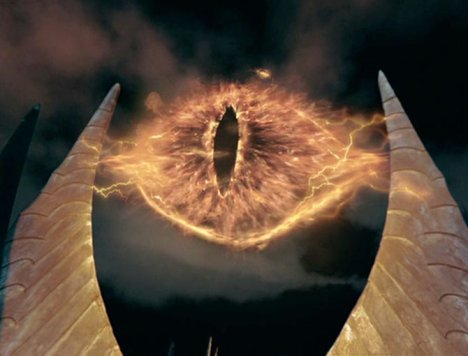
\includegraphics[width=0.35\textwidth]{figures/eye.jpg}};
		\node at (9, -0.3) (node2) {
\includegraphics[width=0.35\textwidth]{figures/teacher.png}};
		\node at (5.5, -3) (node3) {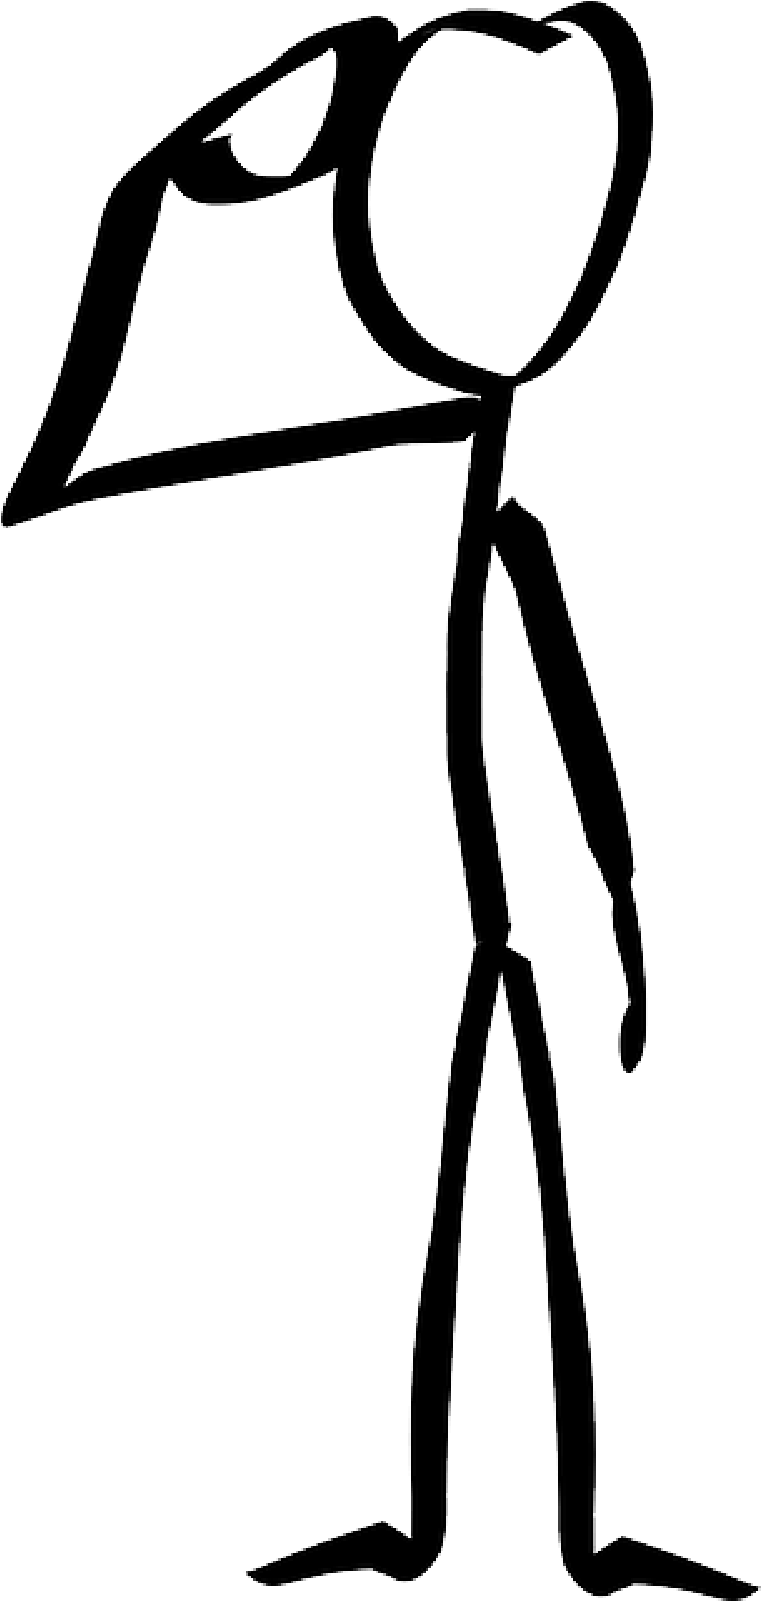
\includegraphics[width=0.10\textwidth]{figures/stick.png}};
		
		\node[notice={(-0.5, -0.3)}, overlay, ellipse callout, text width=2.0cm, align = center] at (4, 2) (node4) {\scriptsize{That's the way I wanted it}};
		\node[notice={(0.4, -0.3)}, overlay, ellipse callout, text width=2.0cm, align = center] at (7, 3) (node4) {\scriptsize{3 is the optimal number of population growth}};
		\node[notice={(-0.5, -0.3)}, overlay, ellipse callout, text width=2.0cm, align = center, fill = white] at (7.75, -0.75) (node4) {\scriptsize{Maybe...but maybe not. I want to see for myself.}};
	\end{tikzpicture}
\end{frame}


%--------------------------%
% How Science Works V      %
%--------------------------%
\begin{frame}[t]
\frametitle{How Science Works}

	\begin{columns}
		\begin{column}{0.4\textwidth}
		
		\end{column}
		
		\begin{column}{0.6\textwidth}
			\textbf{\underline{Hypotheses}}\\
				\begin{itemize}
					\item \emph{\textcolor{red}{Explanatory}} statements about \emph{\textcolor{red}{why}} things are the way they are
					\smallskip
					\item Should lead to clear \emph{\textcolor{red}{predictions}}
					\smallskip
					\item Lead to understanding of multiple observations
					\smallskip
					\item \emph{\textcolor{red}{Must be falsifiable}} (testable)
					\smallskip
					\item Should have more than 1 (process of elimination)
					\smallskip
					\item Are an infinite \# of hypotheses for each observation, but not all equally likely
				\end{itemize}
		\end{column}
	\end{columns}
	
	
\begin{tikzpicture}[overlay]
		\node[draw=green, fill=green!30, ellipse, minimum width = 4cm, minimum height = 3cm, align = center] at (2, 1) (node2) {};
		\node at (2, 2.0) (node3) {Hypotheses};
		\node[draw=myblue2, fill=myblue2!30, ellipse, text width = 2cm, align = center] at (2, 1) (node1) {Observations/ facts};
	\end{tikzpicture}
\end{frame}


%---------------------------%
% How Science Works VI      %
%---------------------------%
\begin{frame}[t]
\frametitle{How Science Works}
\vspace{0.5cm}

	\textcolor{myblue2}{\underline{Hypothesis \#1}: Egg production in species X is limited by available calcium}

	\vspace{0.25cm}

	\textcolor{gray}{\underline{Predictions}:}\\
	\textcolor{gray}{1. Adding Ca to diet will increase egg production}\\
	\textcolor{gray}{2. Reducing Ca in diet will decrease egg production}

	\begin{tikzpicture}[overlay]
		\node[draw=green, fill=green!30, ellipse, minimum width = 4cm, minimum height = 3cm, align = center] at (2, -3.0) (node2) {};
		\node at (2, -2.0) (node3) {Hypotheses};
		\node[draw=myblue2, fill=myblue2!30, ellipse, text width = 2cm, align = center] at (2, -3.0) (node1) {Observations/ facts};
		
		\node[draw=green, fill=green!30, ellipse, minimum width = 4cm, minimum height = 3cm, align = center] at (9, -3.0) (node4) {};
		\node[draw=myblue2, fill=myblue2!30, ellipse, minimum width=2.0cm, minimum height = 1.0cm, align = center] at (9, -3.0) (node5) {
\includegraphics[width=0.15\textwidth]{figures/nest.png}};
	\end{tikzpicture}
\end{frame}


%---------------------------%
% How Science Works VII     %
%---------------------------%
\begin{frame}[t]
\frametitle{How Science Works}
\vspace{0.5cm}

	\textcolor{myblue2}{\underline{Hypothesis \#2}: Egg production in species X is limited by energetic resources}

	\vspace{0.25cm}

	\textcolor{gray}{\underline{Predictions}:}\\
	\textcolor{gray}{1. Adding resources to diet will increase egg production}\\
	\textcolor{gray}{2. Reducing resources in diet will decrease egg production}

	\begin{tikzpicture}[overlay]
		\node[draw=green, fill=green!30, ellipse, minimum width = 4cm, minimum height = 3cm, align = center] at (2, -3.0) (node2) {};
		\node at (2, -2.0) (node3) {Hypotheses};
		\node[draw=myblue2, fill=myblue2!30, ellipse, text width = 2cm, align = center] at (2, -3.0) (node1) {Observations/ facts};
		
		\node[draw=green, fill=green!30, ellipse, minimum width = 4cm, minimum height = 3cm, align = center] at (9, -3.0) (node4) {};
		\node[draw=myblue2, fill=myblue2!30, ellipse, minimum width=2.0cm, minimum height = 1.0cm, align = center] at (9, -3.0) (node5) {
\includegraphics[width=0.15\textwidth]{figures/nest.png}};
	\end{tikzpicture}
\end{frame}


%---------------------------%
% How Science Works VIII    %
%---------------------------%
\begin{frame}[t]
\frametitle{How Science Works}
\vspace{0.5cm}

	\textcolor{myblue2}{\underline{Hypothesis \#3}: Individuals lay different \#s of eggs, but then aliens add/remove them to make it 3}

	\vspace{0.25cm}

	\textcolor{gray}{\underline{Predictions}:}\\
	\textcolor{gray}{1. If we actually watch them lay the eggs, should see different \#s}\\
	\textcolor{gray}{2. If watched 24 hours a day, should see aliens adjusting egg counts}

	\begin{tikzpicture}[overlay]
		\node[draw=green, fill=green!30, ellipse, minimum width = 4cm, minimum height = 3cm, align = center] at (2, -3.0) (node2) {};
		\node at (2, -2.0) (node3) {Hypotheses};
		\node[draw=myblue2, fill=myblue2!30, ellipse, text width = 2cm, align = center] at (2, -3.0) (node1) {Observations/ facts};
		
		\node[draw=green, fill=green!30, ellipse, minimum width = 4cm, minimum height = 3cm, align = center] at (9, -3.0) (node4) {};
		\node[draw=myblue2, fill=myblue2!30, ellipse, minimum width=2.0cm, minimum height = 1.0cm, align = center] at (9, -3.0) (node5) {
\includegraphics[width=0.15\textwidth]{figures/nest.png}};
	\end{tikzpicture}
\end{frame}


%---------------------------%
% How Science Works IX      %
%---------------------------%
\begin{frame}[t]
\frametitle{How Science Works}
\vspace{0.5cm}

	\begin{columns}
		\begin{column}{0.5\textwidth}
			Investigate problem
				\begin{itemize}
					\item Literature
					\smallskip
					\item Experimentation
					\smallskip
					\item Observation
				\end{itemize}
		\end{column}
		
		\begin{column}{0.5\textwidth}
			\begin{center}
				
\includegraphics[width=0.9\textwidth]{figures/science3.jpg}
			\end{center}
		\end{column}
	\end{columns}
\end{frame}


%---------------------------%
% How Science Works X       %
%---------------------------%
\begin{frame}[t]
\frametitle{How Science Works}
\vspace{0.5cm}

	Work through all reasonable hypotheses (that you can)\\
		\medskip
		\begin{itemize}
			\item Ideally, only one is ``left standing'', but not all are mutually exclusive
		\end{itemize}
	
	\vspace{0.25cm}
	
	\begin{center}
		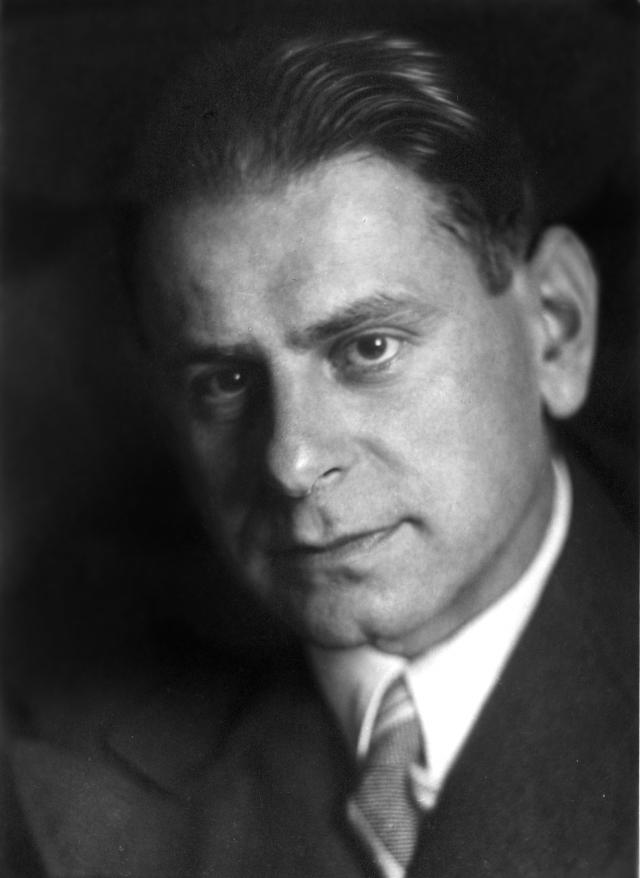
\includegraphics[width=0.3\textwidth]{figures/popper.jpg}\\
		Karl Popper\\
		(1902--1994)
	\end{center}	
\end{frame}


%---------------------------%
% How Science Works XI      %
%---------------------------%
\begin{frame}[t]
\frametitle{How Science Works}

	\begin{tikzpicture}[overlay]
		\node[draw=green, fill=green!30, ellipse, minimum width = 4cm, minimum height = 3cm, align = center] at (2, -5.5) (node1) {};
		\node at (2, -4.5) (node2) {Hypotheses};
		\node[draw=myblue2, fill=myblue2!30, ellipse, text width = 2cm, align = center] at (2, -5.5) (node3) {Observations/ facts};
		
		\node[draw=green, fill=green!30, ellipse, minimum width = 4cm, minimum height = 3cm, align = center] at (9, -5.5) (node4) {};
		\node[draw=myblue2, fill=myblue2!30, ellipse, minimum width=2.0cm, minimum height = 1.0cm, align = center] at (9, -5.5) (node5) {
\includegraphics[width=0.15\textwidth]{figures/nest.png}};
		\node at (6.0, -5.5) (node6) {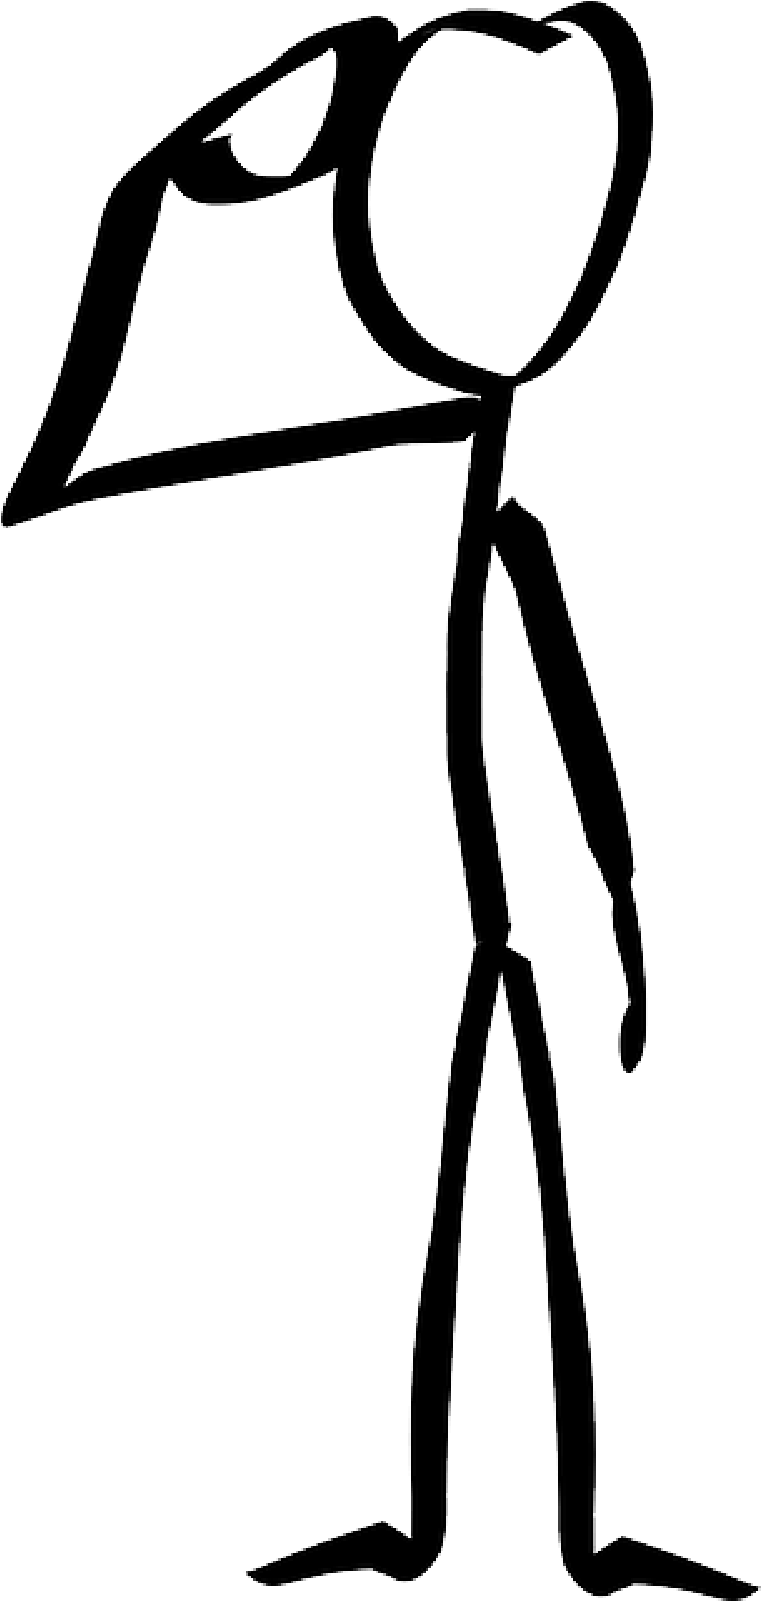
\includegraphics[width=0.10\textwidth]{figures/stick.png}};
		
		\node[text width=2.5cm, align = center] at (2, -2) (node7) {\textcolor{myblue}{\underline{Hypothesis \#1}: Calcium}};
		\node[text width=2.5cm, align = center] at (5.5, -1) (node8) {\textcolor{myblue}{\underline{Hypothesis \#2}: Resources}};
		\node[text width=2.5cm, align = center] at (9, -2) (node9) {\textcolor{myblue}{\underline{Hypothesis \#3}: Aliens}};
	\end{tikzpicture}
\end{frame}


%---------------------------%
% How Science Works XII     %
%---------------------------%
\begin{frame}[t]
\frametitle{How Science Works}

	\begin{tikzpicture}[overlay]
		\node[draw=green, fill=green!30, ellipse, minimum width = 4cm, minimum height = 3cm, align = center] at (2, -5.5) (node1) {};
		\node at (2, -4.5) (node2) {Hypotheses};
		\node[draw=myblue2, fill=myblue2!30, ellipse, text width = 2cm, align = center] at (2, -5.5) (node3) {Observations/ facts};
		
		\node[draw=green, fill=green!30, ellipse, minimum width = 4cm, minimum height = 3cm, align = center] at (9, -5.5) (node4) {};
		\node[draw=myblue2, fill=myblue2!30, ellipse, minimum width=2.0cm, minimum height = 1.0cm, align = center] at (9, -5.5) (node5) {
\includegraphics[width=0.15\textwidth]{figures/nest.png}};
		\node at (6.0, -5.5) (node6) {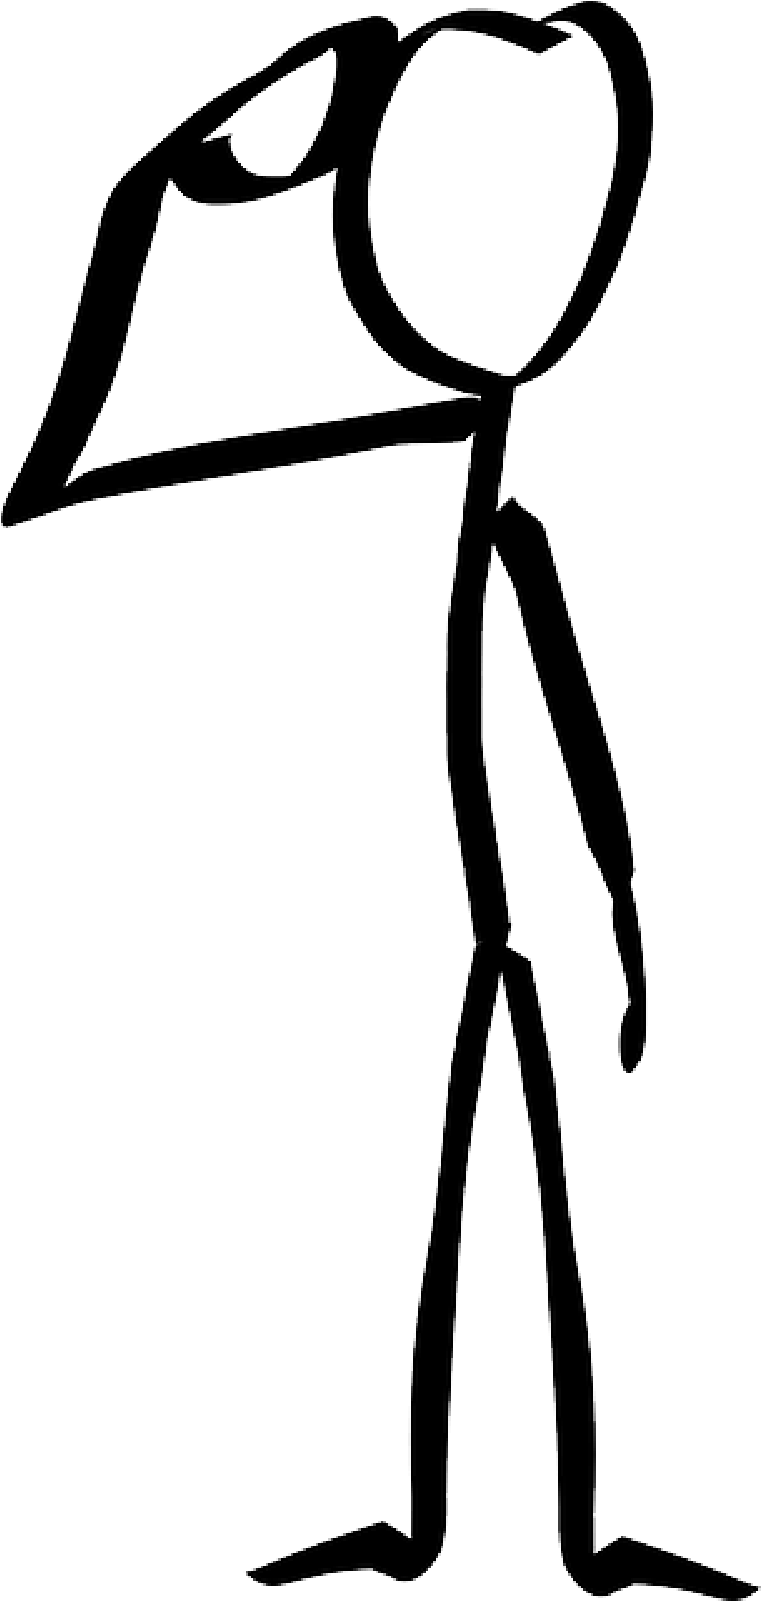
\includegraphics[width=0.10\textwidth]{figures/stick.png}};
		
		\node[text width=2.5cm, align = center] at (2, -2) (node7) {\textcolor{myblue}{\underline{Hypothesis \#1}: Calcium}};
		\node[text width=2.5cm, align = center] at (5.5, -1) (node8) {\textcolor{myblue}{\underline{Hypothesis \#2}: Resources}};
		\node[text width=2.5cm, align = center] at (9, -2) (node9) {\textcolor{myblue}{\underline{Hypothesis \#3}: Aliens}};
		
		\node at (2, -2) (node10) {
\includegraphics[width=0.10\textwidth]{figures/no.png}};
		\node at (9, -2) (node11) {
\includegraphics[width=0.10\textwidth]{figures/no.png}};
	\end{tikzpicture}
\end{frame}


%---------------------------%
% How Science Works XIII    %
%---------------------------%
\begin{frame}[t]
\frametitle{How Science Works}
\vspace{0.5cm}

	\begin{columns}
		\begin{column}{0.6\textwidth}
			Submit your work for peer review\\
			\medskip
				\begin{itemize}
					\item Reasonable hypotheses
					\smallskip
					\item Appropriate methods
					\smallskip
					\item Appropriate interpretation
					\smallskip
					\item \ldots
				\end{itemize}
		\end{column}
		
		\begin{column}{0.4\textwidth}
			\begin{center}
				
\includegraphics[width=0.9\textwidth]{figures/science3.jpg}
			\end{center}
		\end{column}
	\end{columns}
\end{frame}


%---------------------------%
% How Science Works XIV     %
%---------------------------%
\begin{frame}[t]
\frametitle{How Science Works}
\vspace{0.5cm}

	\begin{columns}
		\begin{column}{0.6\textwidth}
			Submit your work for peer review\\
			\medskip
				\begin{itemize}
					\item Reasonable hypotheses
					\smallskip
					\item Appropriate methods
					\smallskip
					\item Appropriate interpretation
					\smallskip
					\item \ldots
				\end{itemize}
		\end{column}
		
		\begin{column}{0.4\textwidth}
			\begin{center}
				
\includegraphics[width=0.9\textwidth]{figures/science3.jpg}\\
			\end{center}
		\end{column}
	\end{columns}
	
	\vspace{0.5cm}
	Adds to our collective understanding of the world\\
	\bigskip
	Now other people can focus on other hypotheses
\end{frame}


%--------------------------%
% How Science Works XV     %
%--------------------------%
\begin{frame}[t]
\frametitle{How Science Works}
\vspace{0.5cm}

	\begin{columns}
		\begin{column}{0.4\textwidth}
		
		\end{column}
		
		\begin{column}{0.6\textwidth}
			\textbf{\underline{Theories}}\\
				\begin{itemize}
					\item General/major \emph{\textcolor{red}{explanatory statements}} that explain many \emph{hypotheses}
					\smallskip
					\item Lead to understanding of multiple hypotheses
				\end{itemize}
		\end{column}
	\end{columns}
	
	\begin{tikzpicture}[overlay]
		\node[draw=red, fill=red!30, ellipse, minimum width = 5cm, minimum height = 4cm, align = center] at (2, -2.0) (node4) {};
		\node[draw=green, fill=green!30, ellipse, minimum width = 4cm, minimum height = 3cm, align = center] at (2, -2.0) (node2) {};
		\node at (2, -1.0) (node3) {Hypotheses};
		\node[draw=myblue2, fill=myblue2!30, ellipse, text width = 2cm, align = center] at (2, -2.0) (node1) {Observations/ facts};
		\node at (2, -0.25) (node5) {Theories};
	\end{tikzpicture}
\end{frame}


%--------------------------%
% How Science Works XVI    %
%--------------------------%
\begin{frame}[t]
\frametitle{How Science Works}

	\begin{tikzpicture}[overlay]
		%--- Theories ---%
		\node[draw=red, fill=red!30, ellipse, minimum width = 2cm, minimum height = 1.5cm] at (6.5, -1.0) (node1) {};
		\node at (1.5, -1.0) (node2) {Theories};
		
		%--- Hypotheses ---%
		\node[draw=green, fill=green!30, ellipse, minimum width = 1.5cm, minimum height = 1.0cm] at (4.5, -3.5) (node3) {};
		\node[draw=green, fill=green!30, ellipse, minimum width = 1.5cm, minimum height = 1.0cm] at (6.5, -3.5) (node4) {};
		\node[draw=green, fill=green!30, ellipse, minimum width = 1.5cm, minimum height = 1.0cm] at (8.5, -3.5) (node5) {};
		\node at (1.5, -3.5) (node6) {Hypotheses};
		\draw[->, >=latex] (node1) -- (node3);
		\draw[->, >=latex] (node1) -- (node4);
		\draw[->, >=latex] (node1) -- (node5);
		
		%--- Observations ---%
		\node[draw=blue, fill=blue!30, ellipse, minimum width = 0.75cm, minimum height = 0.5cm] at (3.5, -6.0) (node7) {};
		\node[draw=blue, fill=blue!30, ellipse, minimum width = 0.75cm, minimum height = 0.5cm] at (4.5, -6.0) (node8) {};
		\node[draw=blue, fill=blue!30, ellipse, minimum width = 0.75cm, minimum height = 0.5cm] at (5.5, -6.0) (node9) {};
		\node[draw=blue, fill=blue!30, ellipse, minimum width = 0.75cm, minimum height = 0.5cm] at (6.5, -6.0) (node10) {};
		\node[draw=blue, fill=blue!30, ellipse, minimum width = 0.75cm, minimum height = 0.5cm] at (7.5, -6.0) (node11) {};
		\node[draw=blue, fill=blue!30, ellipse, minimum width = 0.75cm, minimum height = 0.5cm] at (8.5, -6.0) (node12) {};
		\node[draw=blue, fill=blue!30, ellipse, minimum width = 0.75cm, minimum height = 0.5cm] at (9.5, -6.0) (node13) {};
		\node[text width = 2cm, align = center] at (1.5, -6.0) (node14) {Observations/ facts};
		\draw[->, >=latex] (node3) -- (node7);
		\draw[->, >=latex] (node3) -- (node8);
		\draw[->, >=latex] (node4) -- (node9);
		\draw[->, >=latex] (node4) -- (node10);
		\draw[->, >=latex] (node4) -- (node11);
		\draw[->, >=latex] (node5) -- (node12);
		\draw[->, >=latex] (node5) -- (node13);
	\end{tikzpicture}
\end{frame}


%--------------------------%
% How Science Works XVII   %
%--------------------------%
\begin{frame}[t]
\frametitle{How Science Works}
\vspace{0.5cm}

	\textcolor{myblue}{\underline{Theory}: Natural selection - individuals have evolved to maximize their reproductive success given their environment (egg \# maximizes reproductive ``output'' given the resources available)}
	
	\vspace{0.25cm}
	
	\textcolor{gray}{\underline{Hypothesis \#2}: Resources}
	
	\begin{tikzpicture}[overlay]
		\node[draw=red, fill=red!30, ellipse, minimum width = 5cm, minimum height = 4cm, align = center] at (2, -3.0) (node4) {};
		\node[draw=green, fill=green!30, ellipse, minimum width = 4cm, minimum height = 3cm, align = center] at (2, -3.0) (node2) {};
		\node at (2, -2.0) (node3) {Hypotheses};
		\node[draw=myblue2, fill=myblue2!30, ellipse, text width = 2cm, align = center] at (2, -3.0) (node1) {Observations/ facts};
		\node at (2, -1.25) (node5) {Theories};
		
		\node[draw=red, fill=red!30, ellipse, minimum width = 5cm, minimum height = 4cm, align = center] at (9, -3.0) (node6) {};
		\node[draw=green, fill=green!30, ellipse, minimum width = 4cm, minimum height = 3cm, align = center] at (9, -3.0) (node7) {};
		\node[draw=myblue2, fill=myblue2!30, ellipse] at (9, -3.0) (node8) {
\includegraphics[width=0.15\textwidth]{figures/nest.png}};
	\end{tikzpicture}
\end{frame}


%---------------------------%
%  Theory vs fact           %
%---------------------------%
\begin{frame}[t]
\frametitle{Theory vs Fact in Science}
\vspace{0.5cm}

	\textcolor{myblue}{\textbf{THEORY}}\\
	
	\vspace{0.25cm}
	
	\underline{General Public}:\\
	``An idea. Something not yet proven''.\\
	\emph{e.g.,} ``Evolution is \emph{only} a theory''
	
	\pause
	
	\vspace{0.5cm}
	
	\underline{In Science}:\\
	``A statement of what are held to be the general laws, principles, or causes of something known or observed''.\\
\end{frame}


%---------------------------%
%  Theory vs fact II        %
%---------------------------%
\begin{frame}[t]
\frametitle{Theory vs Fact in Science}
\vspace{0.5cm}

	\textcolor{myblue}{\underline{Fact}:} Gravity exists - things fall\\
	
	\vspace{0.25cm}
	
	\textcolor{myblue}{\underline{Theory of Gravity}:} Our explanation/understanding of why and how things fall\\
	
		\begin{center}
			\rule{0.3\textwidth}{0.5pt}
		\end{center}
		
	\vspace{0.5cm}
	
	\textcolor{myblue}{\underline{Fact}:} Evolution occurs - things evolve\\
	
	\vspace{0.25cm}
	
	\textcolor{myblue}{\underline{Theory of Evolution}:} Our explanation/understanding of why and how things evolve (\emph{e.g.,} natural selection)\\
\end{frame}


%---------------------------%
%  Theory vs fact III       %
%---------------------------%
\begin{frame}[t]
\frametitle{Theory vs Fact in Science}
\vspace{0.5cm}

	\begin{center}
		\textcolor{myblue}{Some other theories in science:}\\
	\end{center}
	
	\vspace{0.25cm}
	
	\begin{columns}
		\begin{column}{0.33\textwidth}
			\begin{center}
				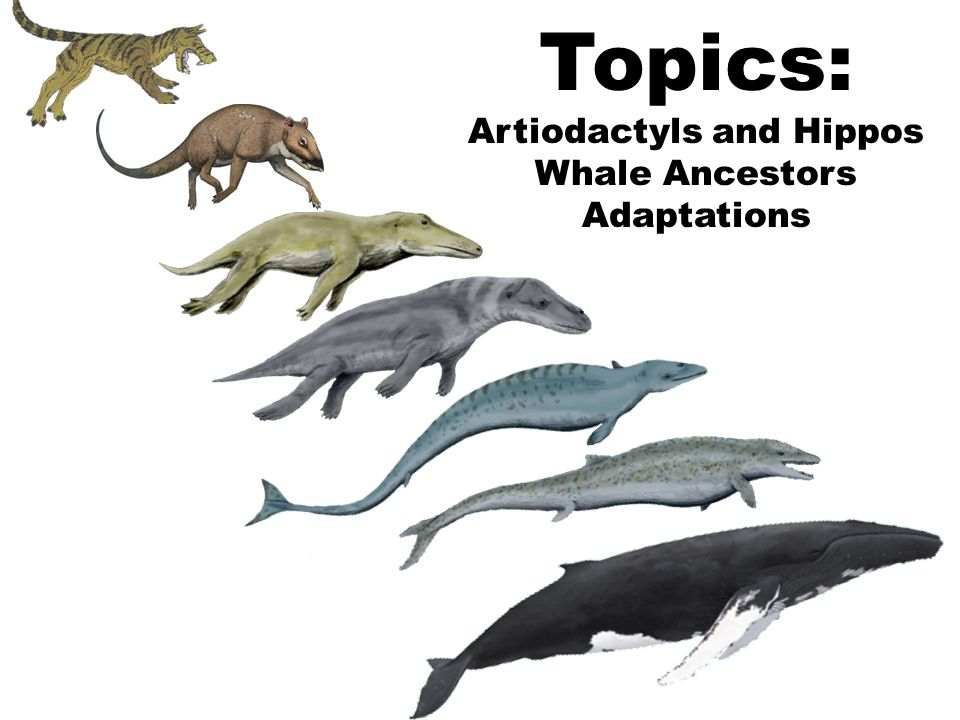
\includegraphics[width=0.9\textwidth]{figures/evolution.jpg}\\
				\vspace{1.0cm}
				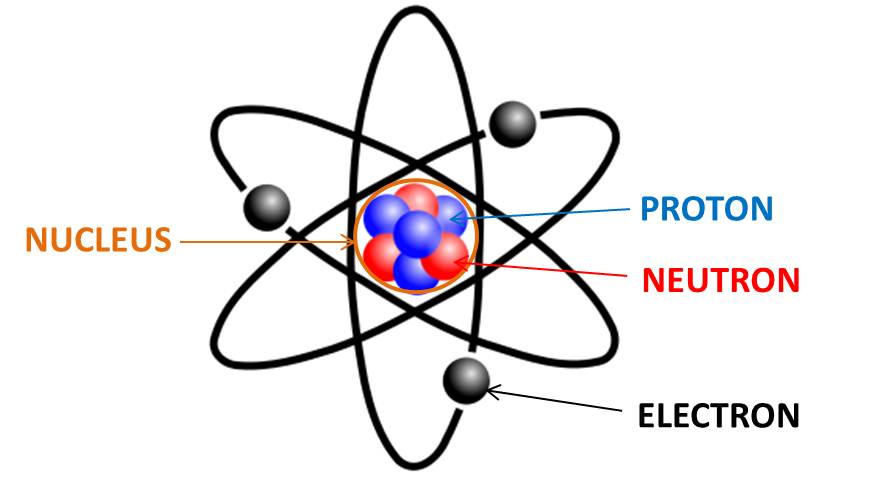
\includegraphics[width=0.9\textwidth]{figures/atom.jpg}\\
			\end{center}
		\end{column}
		
		\begin{column}{0.33\textwidth}
			\begin{center}
				Theory of gravity\\
				\bigskip
				Theory of evolution\\
				\bigskip
				Theory of relativity\\
				\bigskip
				Atomic theory
			\end{center}
		\end{column}
		
		\begin{column}{0.33\textwidth}
			\begin{center}
				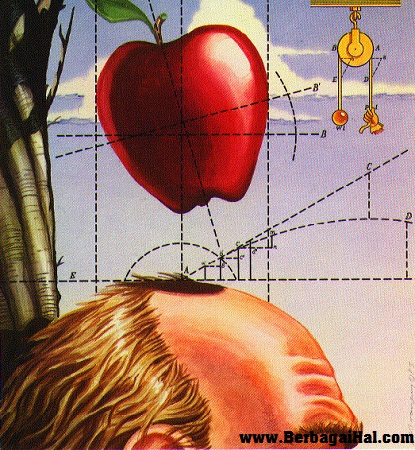
\includegraphics[width=0.7\textwidth]{figures/gravity2.jpg}\\
				\vspace{1.0cm}
				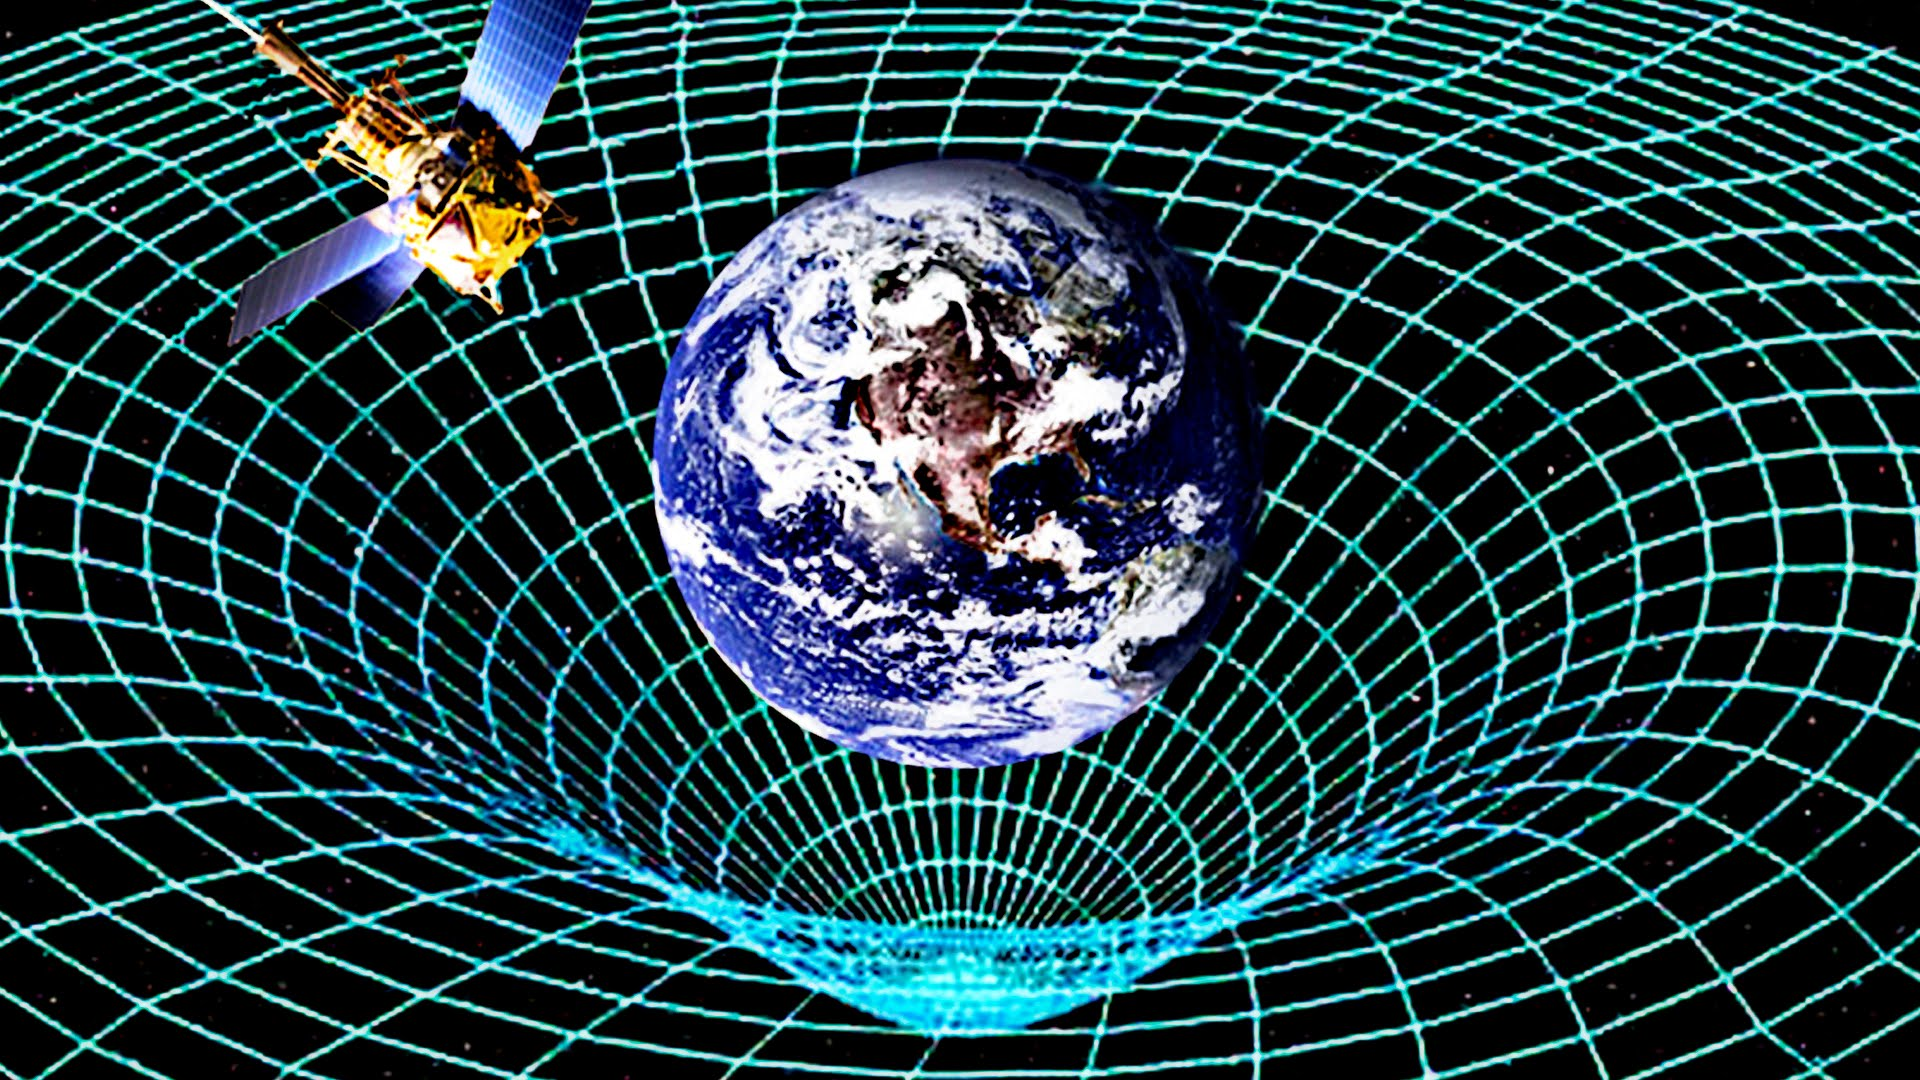
\includegraphics[width=0.9\textwidth]{figures/gravity.jpg}\\
			\end{center}
		\end{column}
	\end{columns}
\end{frame}


%---------------------------%
%  Theory vs fact IV        %
%---------------------------%
\begin{frame}[t]
\frametitle{Theory vs Fact in Science}

	\begin{tikzpicture}[overlay]
		\node at (2, -0.5) (node1) {Fact};
		\node at (2, -2.0) (node2) {Theory};
		\node at (2, -3.5) (node3) {Hypothesis};
		\node at (2, -5.0) (node4) {Guess};
		\node at (7, -3.0) (node5) {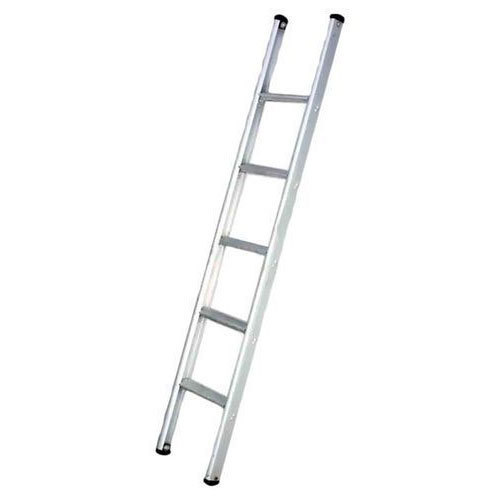
\includegraphics[width=0.55\textwidth]{figures/ladder.jpeg}};
	\end{tikzpicture}	
\end{frame}


%---------------------------%
%  Theory vs fact V         %
%---------------------------%
\begin{frame}[t]
\frametitle{Theory vs Fact in Science}

	\begin{tikzpicture}[overlay]
		\node at (2, -0.5) (node1) {Fact};
		\node at (2, -2.0) (node2) {Theory};
		\node at (2, -3.5) (node3) {Hypothesis};
		\node at (2, -5.0) (node4) {Guess};
		\node at (7, -3.0) (node5) {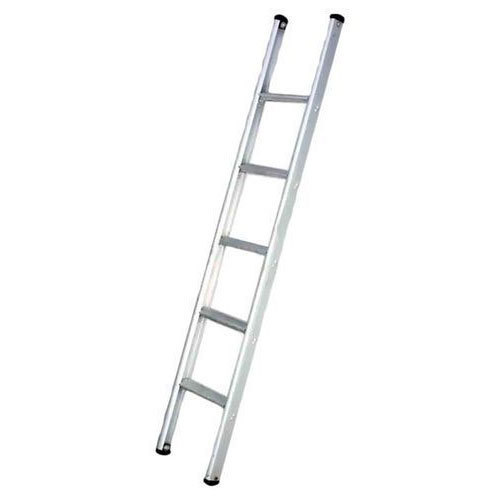
\includegraphics[width=0.55\textwidth]{figures/ladder.jpeg}};
		\node at (5, -3.0) (node5) {
\includegraphics[width=0.65\textwidth]{figures/no.png}};
	\end{tikzpicture}	
\end{frame}


%---------------------------%
%  Theory vs fact VI        %
%---------------------------%
\begin{frame}[t]
\frametitle{Theory vs Fact in Science}
\vspace{0.5cm}
	
	\begin{center}
		Facts and theories are different things, \textcolor{red}{NOT}\\ different rungs on a hierarchy\\
		
		\vspace{0.7cm}
		
		Facts are the world's data, theories are structures of \\ideas that explain and interpret facts
	\end{center}
\end{frame}


%---------------------------%
%  Theory vs fact VII       %
%---------------------------%
\begin{frame}[t]
\frametitle{Theory vs Fact in Science}
\vspace{0.5cm}
	
	``Evolution is \emph{only} a theory'' is \textcolor{red}{not} a valid criticism\\
	\smallskip
		\begin{itemize}
			\item Indicates a misunderstanding of terminology
			\smallskip
			\item Suggests theories can become something else if more evidence/support is obtained (which they can't)
		\end{itemize}
\end{frame}


%---------------------------%
%  Nature of Science I      %
%---------------------------%
\begin{frame}[t]
\frametitle{Nature of Science}
\vspace{0.5cm}

	Scientifically, can we be 100\% sure of a hypothesis/theory?\\
	
	\pause
	
	\begin{center}
		\textcolor{myblue}{Absolutely not! Why not?}\\
	\end{center}
	\vspace{0.5cm}
	
	\pause
	
	World is very complicated\\
		\smallskip
		\begin{itemize}
			\item Old hypotheses/theories constantly revised
			\smallskip
			\item New hypotheses/theories constantly developed\\
		\end{itemize}
	
	\vspace{0.5cm}
	
	Current understanding influenced by\\
		\smallskip
		\begin{itemize}
			\item Previous knowledge
			\smallskip
			\item Culture
			\smallskip
			\item Technology
			\smallskip
			\item \ldots
		\end{itemize}	
\end{frame}


%---------------------------%
%  Nature of Science II     %
%---------------------------%
\begin{frame}[t]
\frametitle{Example: Gravity}
\vspace{0.25cm}

	\begin{columns}
		\begin{column}{0.3\textwidth}
			\begin{center}
				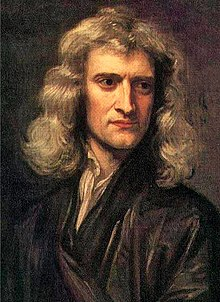
\includegraphics[width=0.6\textwidth]{figures/newton.jpg}
			\end{center}
		\end{column}
		
		\begin{column}{0.7\textwidth}
			Newton first described gravity scientifically
				\begin{itemize}
					\item Explained the majority of observations that most people had\\
				\end{itemize}
		\end{column}
	\end{columns}
	
	\vspace{0.25cm}
	
	\begin{center}
		As telescopes developed, some people noticed some orbits didn't quite agree with Newtonian expectations.\\
	\end{center}
	
	\vspace{0.25cm}

	\begin{columns}
		\begin{column}{0.3\textwidth}
			\begin{center}
				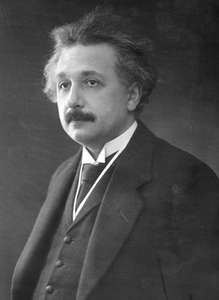
\includegraphics[width=0.6\textwidth]{figures/einstein.jpg}
			\end{center}
		\end{column}
		
		\begin{column}{0.7\textwidth}
			Einstein developed a new theory that explained things better
				\begin{itemize}
					\item \textcolor{myblue}{Einstein's theory will undoubtedly be revised}
				\end{itemize}
		\end{column}
	\end{columns}
\end{frame}


%---------------------------%
%  Nature of Science III    %
%---------------------------%
\begin{frame}[t]
\frametitle{Nature of Science}
\vspace{0.5cm}

	Can't ever ``prove'' a hypothesis\\
	
	\vspace{0.25cm}
	
	Can only reject all other potential explanations (that we can think of)
	
	\vspace{0.5cm}
	
	\begin{columns}
		\begin{column}{0.3\textwidth}
			\begin{center}
				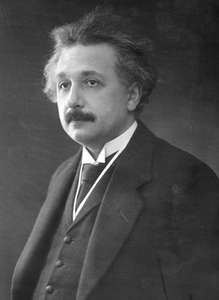
\includegraphics[width=0.6\textwidth]{figures/einstein.jpg}
			\end{center}
		\end{column}
		
		\begin{column}{0.7\textwidth}
			\emph{\textcolor{myblue}{No amount of experimentation can ever prove me right; a single experiment can prove me wrong.}}
		\end{column}
	\end{columns}
\end{frame}


%---------------------------%
%  Nature of Science IV     %
%---------------------------%
\begin{frame}[t]
\frametitle{Nature of Science}
\vspace{0.5cm}

	If done correctly, science is self-correcting\\
	
	\vspace{0.5cm}
	
	Only way we have of improving our understanding of the world\\
	
	\vspace{0.5cm}
	
	\begin{center}
		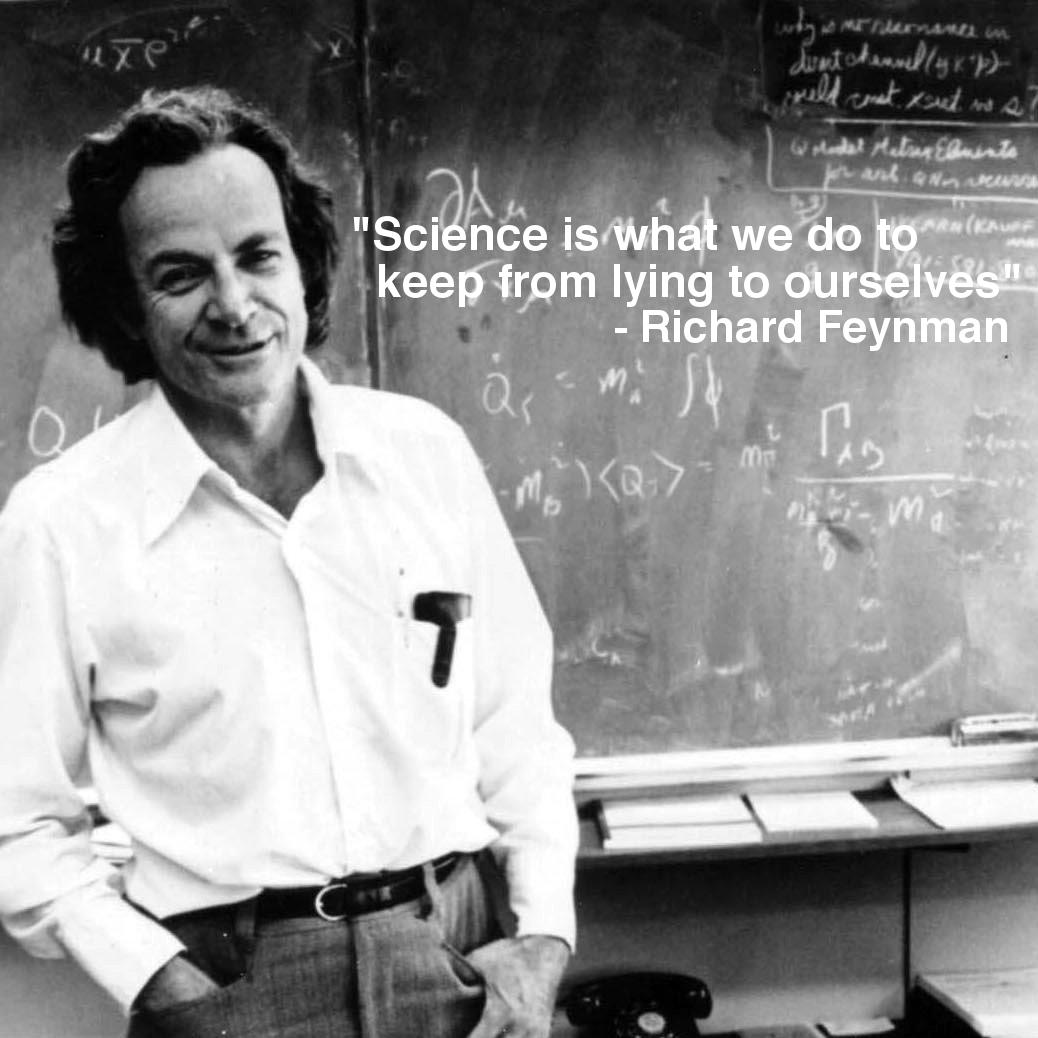
\includegraphics[width=0.5\textwidth]{figures/feynman.jpg}
	\end{center}
\end{frame}


%---------------------------%
%  Nature of Science V      %
%---------------------------%
\begin{frame}[t]
\frametitle{Nature of Science}
\vspace{0.5cm}

	If done correctly, science is self-correcting\\
	
	\vspace{0.5cm}
	
	Only way we have of improving our understanding of the world\\
	
	\vspace{0.5cm}
	
	\begin{center}
		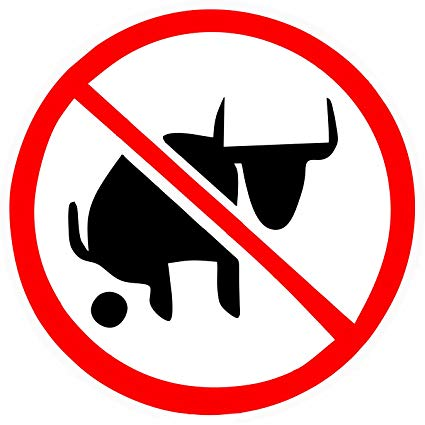
\includegraphics[width=0.35\textwidth]{figures/bullshit.jpg}
	\end{center}
\end{frame}

	
%---------------------------%
% Questions                 %
%---------------------------%
\begin{frame}
	\begin{center}
		\Huge{\textcolor{myblue}{Questions?}}
	\end{center}	
\end{frame}


%---------------------------%
% Case Studies              %
%---------------------------%
\begin{frame}[t]
\frametitle{Case Studies}
\vspace{0.25cm}

	\begin{center}
		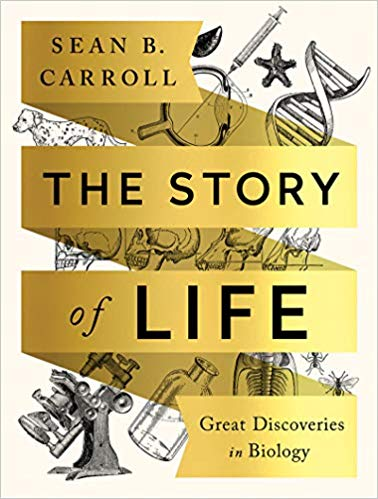
\includegraphics[width=0.3\textwidth]{../Topic1-Introduction/figures/carroll.jpg}
	\end{center}
\end{frame}


%---------------------------%
% Case Study #1             %
%---------------------------%
\begin{frame}[t]
\frametitle{Case Study \#1}
\framesubtitle{Cause of gastritis and ulcers}

	\begin{columns}
		\begin{column}{0.4\textwidth}
			\begin{center}
				Robin Warren (left) \& Barry Marshall (right)\\
				\vspace{0.2cm}
				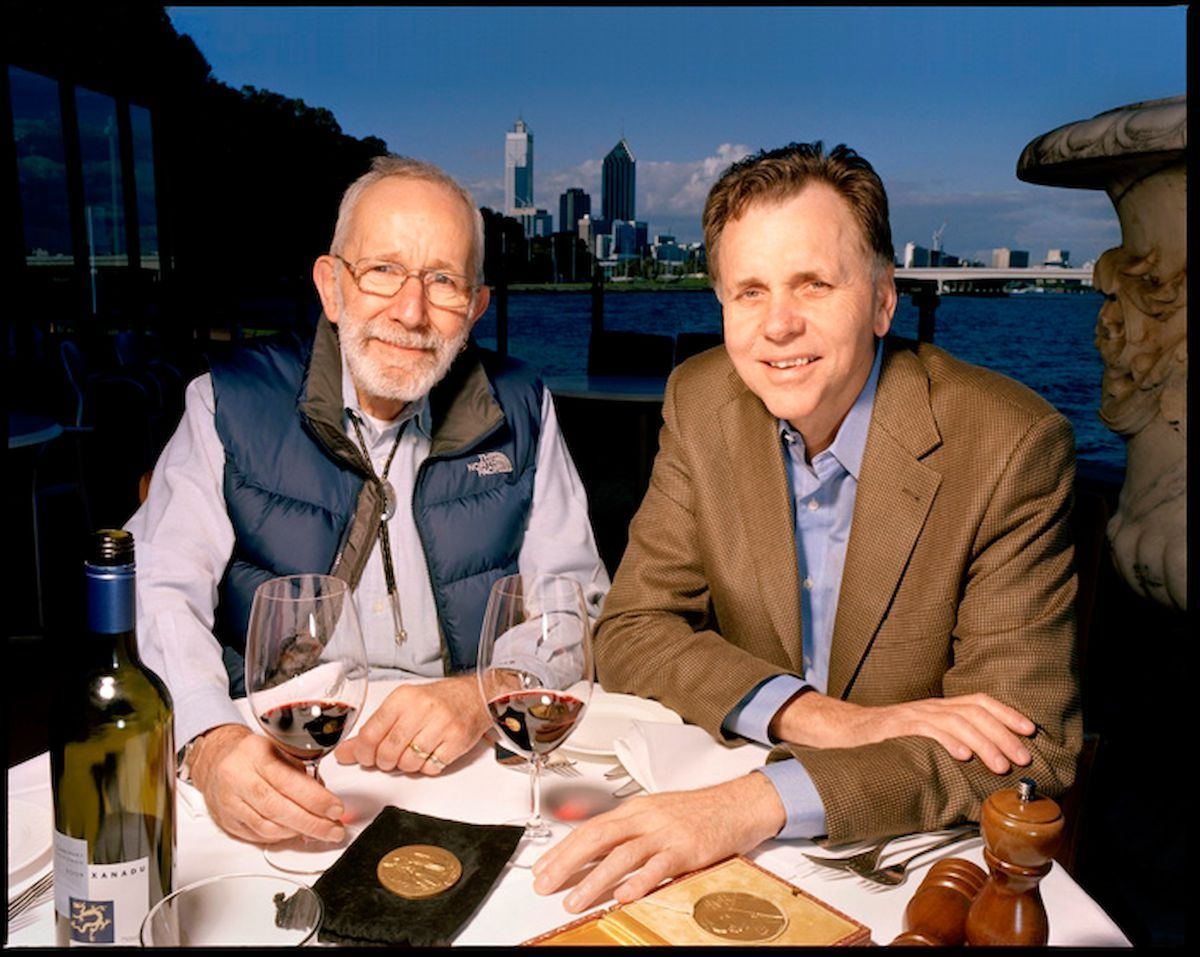
\includegraphics[width=1.0\textwidth]{figures/warren.jpg}\\
				\vspace{0.2cm}
				Nobel Prize in 2005
			\end{center}
		\end{column}
		
		\begin{column}{0.6\textwidth}
			\begin{center}
				\includegraphics[width=0.9\textwidth]{figures/ulcer.pdf}
			\end{center}
		\end{column}
	\end{columns}
\end{frame}


%---------------------------%
% Case Study #2 I           %
%---------------------------%
\begin{frame}[t]
\frametitle{Case Study \#2}
\framesubtitle{Vaccines and autism}

	\begin{reference}{4mm}{92mm}
		\rule{1.5cm}{0.25pt}\\
		Wakefield et al. (1998) \emph{The Lancet} \textbf{351}: 637--641.
	\end{reference}
	
	\begin{center}
		\includegraphics[width=0.8\textwidth]{figures/wakefield_paper.png}\\
		\vspace{0.5cm}
		\includegraphics[width=0.2\textwidth]{figures/wakefield.jpg}
	\end{center}
\end{frame}


%---------------------------%
% Case Study #2 II           %
%---------------------------%
\begin{frame}
\frametitle{Case Study \#2}
\framesubtitle{Vaccines and autism}

	\begin{center}
		\includegraphics[width=0.7\textwidth]{figures/wakefield_paper2.png}
	\end{center}
\end{frame}


%---------------------------%
% Case Study #2 III         %
%---------------------------%
\begin{frame}
\frametitle{Case Study \#2}
\framesubtitle{Vaccines and autism}

	\begin{reference}{4mm}{92mm}
		\rule{1.5cm}{0.25pt}\\
		Taylor et al. (1999) \emph{The Lancet} \textbf{353}: 2026--2029.
	\end{reference}

	\begin{center}
		\includegraphics[width=0.8\textwidth]{figures/taylor_paper.png}\\
		\vspace{0.5cm}
		\includegraphics[width=0.2\textwidth]{figures/taylor.jpeg}
	\end{center}
\end{frame}


%---------------------------%
% Case Study #2 IV          %
%---------------------------%
\begin{frame}
\frametitle{Case Study \#2}
\framesubtitle{Vaccines and autism}

	\begin{center}
		\includegraphics[width=0.45\textwidth]{figures/wakefield_paper3.png}
	\end{center}
\end{frame}

	
\end{document}